
\documentclass[11pt,a4paper]{article}
\usepackage[T1]{fontenc}
\usepackage[utf8]{inputenc}
\usepackage{authblk}
\usepackage[english]{babel}
\usepackage{fancyhdr}
\usepackage{subfig}
\usepackage{float}

\newcommand*\samethanks[1][\value{footnote}]{\footnotemark[#1]}
\title{Transition Form Factors of the $\eta^{\prime}$ and $\phi$ Mesons with CLAS12}
\date{}
\author[1]{Michael C. Kunkel\thanks{Contact person, email: m.kunkel@fz-juelich.de}\thanks{Spokesperson}}
\author[1]{Daniel Lersch}
\author[1]{Jim Ritman\samethanks}
\author[1]{Susan Schadmand\samethanks}
\author[1]{Xinying Song}
\affil[1]{Forschungszentrum J\"ulich, J\"ulich (Germany)}

\renewcommand\Authands{, }

\fancypagestyle{firststyle}
{
	\fancyhf{}
	\renewcommand{\headrulewidth}{0pt}
	\fancyhead[C]{\Large A CLAS Proposal for PAC44}
}


\def\etaP{\eta^{\prime}}
\def\grpath{figures}
\newcommand{\abbr}[1]{\textsc{\texttt{#1}}}
%%%% environment to highlight text that has changed in version 2.0
\newenvironment{v2}{\color{BrickRed}}{\ignorespacesafterend}

\newlength{\figwidth}
\setlength{\figwidth}{0.9\columnwidth}

\newlength{\qfigheight}
\setlength{\qfigheight}{0.25\textheight}

\newlength{\hfigheight}
\setlength{\hfigheight}{0.5\textheight}

\newcommand{\abbr}[1]{\textsc{\texttt{#1}}}
\newcommand{\desg}[1]{\textit{#1}}
\newcommand{\prog}[1]{\texttt{#1}}

\newcommand{\system}[1]{\abbr{#1}}
\newcommand{\bank}[1]{\abbr{#1}}

\newcommand{\todo}[1]{\textbf{\textcolor{Orange}{#1}}}

\def\Lqcd{\mathcal{L}_{\mathtt{QCD}}}
\def\qfield{\psi}
\def\qbarfield{\overline{\psi}}

\def\th{\textsuperscript{th}}
\def\ith{i\th}

\def\um{{\textmu}m}
\def\d{\mathrm{d}}

%\def\coloronline{(Color online.)\ }
\def\coloronline{}



\newcommand{\particle}[2]{\text{#1\ifthenelse{\equal{#2}{}}{}{$^{#2}$}}}

\newcommand{\e}[1][]{\particle{e}{#1}}
\newcommand{\π}[1][]{\particle{π}{#1}}
\newcommand{\K}[1][]{\particle{K}{#1}}



%%% quarks
\def\uquark{\mathbf{u}}
\def\dquark{\mathbf{d}}
\def\squark{\mathbf{s}}


%%% particles
\def\photon{\text{γ}}
\def\electron{\mathrm{e}^-}
\def\positron{\mathrm{e}^+}
\def\nucleon{\mathrm{N}}
\def\proton{\mathrm{p}}
\def\neutron{\mathrm{n}}
\def\pion{\text{π}}
\def\kaon{\mathrm{K}}
\def\hyperon{\text{Y}}
\def\etameson{\text{η}}
\def\omegameson{\text{ω}}
\def\phimeson{\text{φ}}
\def\rhomeson{\text{ρ}}

\def\piplus{\pion^+}
\def\piminus{\pion^-}
\def\Kplus{\kaon^+}
\def\Kminus{\kaon^-}
\def\Kshort{\kaon^0}
\def\pip{$\pion^+$ }
\def\piz{$\pion^0$ }
\def\pim{$\pion^-$ }
\def\pippim{$\pion^+\pion^-$ }
\def\Ks{$\kaon_s$ }
%%% systems
\def\rf{\mathtt{RF}}
\def\tg{\mathtt{TAG}}
\def\tgrf{\tg_{\rf}}
\def\tof{\mathtt{TOF}}
\def\st{\mathtt{ST}}
\def\beam{\mathrm{beam}}
\def\adc{\mathtt{ADC}}
\def\tdc{\mathtt{TDC}}

%%% descriptives
\def\prop{\mathrm{prop}}
\def\trigoffset{\mathrm{trigger-offset}}
\def\pid{\mathtt{PID}}
\def\vtx{\mathrm{vtx}}

%%% dE/dx
\def\dEdx{\frac{\mathrm{d}E}{\mathrm{d}x}}
\def\dEdxvar{\mathrm{d}E/\mathrm{d}x}

%%% Beta
\def\betasttof{\beta_{\st - \tof}}
\def\betatof{\beta_\tof}
\def\betapid{\beta_\pid}
\def\gammatof{\gamma_\tof}
\def\gammapid{\gamma_\pid}

%%% TAGGER and RF related times
\def\trf{t_\rf}
\def\ttg{t_\tg}
\def\ttgrf{t_{\tg,\rf}}
\def\tpho{t_\mathrm{photon}}
\def\tprop{t_\prop}
\def\ttrigoffset{t_\trigoffset}

\def\tphotgrf{\tpho^{\tg,\rf}}
\def\tphotofpid{\tpho\left(\tof\right)}
\def\tphostpid{\tpho\left(\st\right)}

%%% delta tpho
\def\dtpho{\Delta\tpho}
\def\dtphotofpid{\dtpho\left(\tof-\tg\right)}
\def\dtphosttof{\dtpho\left(\tof-\st\right)}
\def\dtphostpid{\dtpho\left(\st-\tg\right)}

%% particle specific tpho (TOF)
\def\tphotofpidkpf{\tpho\left(\tof,\KplusFast\right)}
\def\tphotofpidkps{\tpho\left(\tof,\KplusSlow\right)}
\def\dtphotofpidkpf{\dtpho\left(\tof-\tg,\KplusFast\right)}
\def\dtphotofpidkps{\dtpho\left(\tof-\tg,\KplusSlow\right)}
\def\dtphotofpidkpkp{\dtpho\left(\tof,\KplusFast-\KplusSlow\right)}

%% particle specific tpho (ST)
\def\dtphostpidkpf{\dtpho\left(\tof-\tg,\KplusFast\right)}
\def\dtphostpidkps{\dtpho\left(\tof-\tg,\KplusSlow\right)}

%%% BEAM energy
\def\Epid{E_\pid}
\def\Ebeam{E_\beam}

%%% TOF Energy deposit
\def\Edeptof{\dEdx\left(\tof\right)}
\def\Edeptofvar{\dEdxvar\left(\tof\right)}


%%% path lengths
\def\lst{\ell_\st}
\def\ltof{\ell_\tof}
\def\lsttof{\ell_{\st-\tof}}

%%% raw subsystem times
\def\tst{t_\st}
\def\ttof{t_\tof}
\def\tsttof{\tsttof}

%%% vertex times
\def\tv{t_\vtx}
\def\tvtgrf{\tv^{\tg,\rf}}
\def\tvtofpid{\tv^\tof}
\def\tvstpid{\tv^\st}

%%% delta vertex times
\def\dtvst{\Delta t_\mathrm{vtx}(\mathtt{TOF-ST})}
\def\dtvpid{\Delta t_\mathrm{vtx}(\mathtt{TOF-PID})}

%%% z position
\def\zv{z_\mathrm{vtx}}
\def\ztgt{z_\mathrm{tgt}}

%%% mass
\def\mtof{m_\tof}
\def\mbook{m_\mathrm{book}}

\def\adcst{\mathtt{ADC}_{\mathtt{ST}}}

\def\M{\mathrm{M}}
\def\MM{\mathrm{MM}}

\def\mmkk{\MM\left(\Kplus\Kplus\right)}

\newcommand{\bra}[1]{\left<#1\right|}
\newcommand{\ket}[1]{\left|#1\right>}
\newcommand{\braket}[2]{\left<#1\middle|#2\right>}

\newcommand*\midhrulefill{%
    \leavevmode\leaders\hrule depth-2pt height 2.4pt\hfill\kern0pt
}

% Document starts
\begin{document}
\maketitle
\thispagestyle{firststyle}
\begin{abstract}
	Dalitz decays are radiative decays in which the photon is virtual and subsequently produces an electron positron pair, $P\rightarrow l^+l^-X$. It is an important tool used to reveal the internal structure of hadrons and the interaction mechanisms between photons and hadrons. Furthermore, assuming point-like particles, the electromagnetic interaction is calculable within QED by the Kroll-Wada formula. Transition form factors are deviations from the QED decay rate. They characterize modifications of the point-like photon-meson vertex due to the structure of the meson. For the $\etaP$ meson this deviation represents the internal structure of the meson, while for the $\phi$ meson the deviation represents the transition from $\phi \to \eta$. The transition form factor can be characterized as $\left| F(q^2)\right|$, where $q^2$ is the square of the invariant mass of the lepton pair, and can be determined by comparing QED to what is measured experimentally.
	\\ 
	\indent Measurements with the highest scientific impact on the determination of the transition form factor have been performed in the space-like region ($\mathrm{q}^2<0$) in collider experiments. However, due to experimental limitations (e.g. $\pi^{\pm}$ contamination in lepton sample, low branching fractions, external conversion contamination), transition form factors in the time-like region ($\mathrm{q}^2>0$) have not yet been precisely determined. Recent measurements of the time-like transition form factor for $\etaP \to e^+e^- \gamma$ have been performed by the BESIII collaboration with insufficient statistical precision, therefore the proper theoretical description cannot be determined. 
	\\
	\indent From previous CLAS analyses using the g12 data set, it was preliminarily shown that measurements of the time-like transition form factor were achievable, but without the statistical precision needed to be completive. Therefore, we propose to use CLAS12 to focus on the dilepton decay channels from the reactions $ep\rightarrow e^{\prime}p\etaP$ and $ep\rightarrow e^{\prime}p\phi$, where $\etaP \to e^+e^- \gamma$ and $\phi \rightarrow \eta e^+e^-$. The CLAS12 detector will be used to identify and measure the $e^+e^-$ decay products by means of the High Threshold Cherenkov Counter (HTCC), Pre-Calorimeter (PCAL) and Electromagnetic Calorimeter (EC). The combination of HTCC+PCAL+EC can provide a rejection factor for single $e^\pm/\pi^\pm$ of up to $10^6$ for momenta less than 4.9~GeV/c with $\approx$ 100\% efficiency. For dileptons ($e^+e^-$ pairs), this rejection factor will be $\approx 10^{12}$, which enables dilepton studies for branching ratios $\approx 10^{-9}$. Precise determination of momenta and angles of the $e^+e^-$ decay products  are the key features available to CLAS12. Preliminary studies using the CLAS12 simulation suite have shown that a beam time of 100 days, at full luminosity, will accumulate a data sample at least one order of magnitude larger in statistics, than the most current $\etaP \to e^+e^- \gamma$ and $\phi \rightarrow \eta e^+e^-$ measurement. 
\end{abstract}
%\section{Introduction}
\indent Current measurements on the determination of the transition form factor have been performed in the space-like region ($\mathrm{q}^2<0$) in collider experiments. However, due to experimental limitations (e.g. $\pi^{\pm}$ contamination in lepton sample, low branching fractions, external conversion contamination), transition form factors in the time-like region ($\mathrm{q}^2>0$) have not yet been precisely determined. Recent measurements of the time-like transition form factor for $\etaP \to e^+e^- \gamma$ have been performed by the BESIII collaboration with insufficient statistical precision to distinguish between different theoretical approaches. 
\subsection{Motivation}
While very successful in many aspects, the Standard Model of particle physics (SM)
leaves a few important questions unanswered. On the one hand, it predicts
an amount of matter that survived annihilation after the Big Bang that is many orders
of magnitude less compared to what is observed. In addition, since masses
of matter particles appear as parameters in the SM, it does not provide any understanding
why the values of these masses span so many orders of magnitude.
In addition, within the SM, phenomena like Dark Matter and Dark Energy can not be explained.
These and some more 
issues suggest that there must be physics beyond the SM, and many experiments
world-wide hunt for signals of it. 

One of the currently most promising candidates to provide a signal for physics beyond the SM
is the muon anomaly. It is a low-energy observable, which
can be both measured and computed to high precision~\cite{Jegerlehner:2009ry,Blum:2013xva}.
``The anomaly is defined by $a_\mu = (g-2)/2$, where the Land\`e g-factor is the proportionality constant that relates the spin to the magnetic moment.
 For the muon, as well as for the electron and tauon,
  the anomaly $a$ differs slightly from zero (of order $10^{-3}$)
  because of radiative corrections. In the Standard Model, contributions to the anomaly come from virtual `loops' containing photons and the known massive particles.''~\cite{miller} 
 The present experimental value $a_\mu^{\rm EXP}= 1\ 165\ 920\ 89 (63)\times 10^{-11}$
comes from the BNL E821 experiment~\cite{Bennett:2006fi}.  This value
deviates from the SM prediction by about 3 standard
deviations $\Delta a_\mu^{({\rm EXP-SM})}= (287\pm 80)\times 10^{-11}$~\cite{Davier:2010nc} 
or $= (261\pm 78)\times 10^{-11}$~\cite{Hagiwara:2011af}, depending on how the leading-order
hadronic contributions are evaluated.  While this discrepancy
is not large enough to claim a failure of the SM, it is currently the largest
deviation of a SM prediction from an experimental observable. This
alone justifies the efforts currently taken to improve both the theoretical as well as the experimental value.
New measurements are planned within the next four years at 
Fermilab/USA~\cite{Grange:2015fou} and also at JPARC/Japan~\cite{Saito:2012zz}. The goal
of the measurements is to reduce the uncertainty by a factor of four. 
In parallel the SM prediction needs to be improved in accuracy 
by at least a factor of two to establish a deviation from the SM for the first time.


The largest uncertainty of the SM prediction comes from
the hadronic quantum corrections~\cite{Jegerlehner:2009ry}.
At the level of accuracy that is relevant at the moment the hadronic
contributions can be split up into the hadronic vacuum polarization
(HVP), displayed on the left-hand side of figure \ref{fig:gm2}, and the
hadronic light-by-light scattering (HLbL), displayed in the middle of
Fig.~\ref{fig:gm2}. The most important contribution to the latter
comes from the pseudoscalar pole contributions, displayed explicitly on the right-hand 
side of Fig.~\ref{fig:gm2}. For those one expects that the contribution
should be largely saturated by the lightest exchange particles, namely the 
$\pi^0$, the $\eta$ and the $\eta'$. 
%
\begin{figure}[!h]
	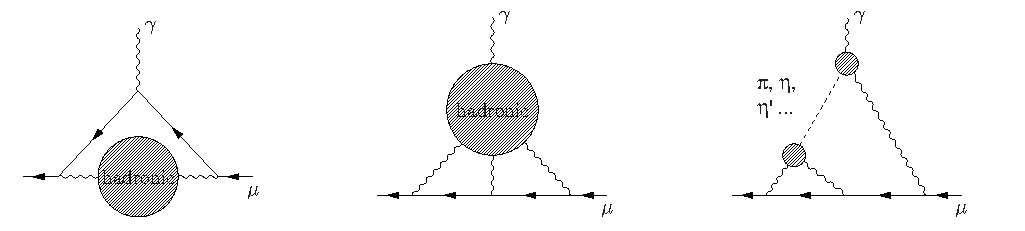
\includegraphics[keepaspectratio,width=1.\textwidth]{figures/intro/hadronicgm2.pdf}
	\caption{Hadronic contributions to $a_\mu$: hadronic vacuum polarization (left diagram), 
		hadronic light-by-light scattering (middle), pion-pole contribution to hadronic light-by-light scattering (right). Full lines with an arrow denote muons, wiggly lines photons, the dashed line a pseudo-scalar meson and shaded blobs a non-pointlike hadronic substructure. The upper blob in the right diagram corresponds to Fig.~\ref{fig:piz.dalitz}, while the lower blob corresponds to the double Dalitz decay. 
	}
	\label{fig:gm2}
\end{figure}

Concerning the SM prediction for $a_\mu$ HLbL is suppressed relative to HVP by one power of the electromagnetic
fine structure constant~\cite{Jegerlehner:2009ry,Bijnens:2007pz}.  
Unfortunately at present it is not possible to straightforwardly 
calculate the contributions shown in Fig.~\ref{fig:gm2} 
from first principles analogously to, e.g., the QED corrections, since
both processes concern low-energy corrections,
i.e.\ non-perturbative physics. Thus the prime candidate for a SM
calculation of hadronic corrections seems to be lattice QCD~\cite{Gattringer:2010zz}. 
However, it is not expected that lattice QCD
results for HPV will reach the required accuracy in the foreseeable future.
For the HLbL only preliminary lattice-QCD calculations have been reported~\cite{Blum:2014oka}.  
In view of the challenges to determine
a four-point function that includes in addition disconnected diagrams
it is not clear yet when a profound lattice calculation with
controlled uncertainties and a reliable error estimate will be
available.

Fortunately there is an alternative way to quantify hadronic corrections. It requires both
theoretical as well as experimental efforts:
Dispersion theory provides a link between particular hadronic cross sections
and $a_\mu$---for a discussion of the HVP in this context see Ref.~\cite{Jegerlehner:2009ry}, while 
for HLbL we refer to Refs.~\cite{Colangelo:2014dfa,Pauk:2014rfa,Colangelo:2014pva,Colangelo:2015ama}.  
In particular for the latter contribution it allows one to calculate from the transition
form factors of the kind $\pi^0$, $\eta$, $\eta'\to \gamma^*\gamma^*$ 
the corresponding piece for the meson pole contribution as displayed in the
right most diagram of Fig.~\ref{fig:gm2}.
The measurements proposed here provide important information towards
the necessary input needed for the evaluation of the HLbL contribution, since
$\eta'\to \gamma^*\gamma$ gives the single off-shell form factor of the $\eta'$
and $\phi\to \eta\gamma$ additionally provides information on the isoscalar
piece of $\eta\to \gamma^*\gamma$ in a different kinematic regime.
Additional information on the  $\eta$ and
$\eta'$ form factors can be found from the dispersive methods outlined in
Refs.~\cite{Adlarson:2011xb,Stollenwerk:2011zz,Hanhart:2013vba,Kubis:2015sga,Xiao:2015uva}.
It  appears to be realistic that this joined effort of theory and experiment
will provide the improvements necessary to push the SM calculation towards
the required accuracy. For the $\etaP$ pole contribution a precision of 15\% on the HLbL correction are feasible.~\cite{Nyffeler}.

\subsection{History}
\indent In the year 1951, Richard Dalitz published a letter~\cite{Dalitz} in which he calculated the rate for the \pizT  decaying into an electron-positron pair (dilepton) and a photon, \pizDal. The calculation assumed that the decay proceeded through a two–photon decay in which one of the photons was virtual and converted into an electron-positron pair.  This kind of reaction is now known as Dalitz decay. The experimental evidence of this decay process was first observed in emulsion plates exposed to the Chicago cyclotron in 1952~\cite{Lord} and a number of experiments performed over the next ten years verified Dalitz’s hypothesis that the \pizDal \ decay resulted from emission of a virtual photon~\cite{Samios,Lindenfeld,Sargent}. A few years later N. Kroll and W. Wada calculated the framework for Dalitz decays within the QED framework~\cite{KrollWada}, and extended the framework to double Dalitz Decays, in which the \pizT decays into two electron-positron pairs via emission of two virtual photons. \\
\indent Throughout the following years, much work was done to extend the framework of Dalitz decays to heavier mesons, such as \etaT, \omT, \etaTP, and \phiT. With numerous experimental data taken, it was shown that the shape of the dilepton mass spectrum deviated from the QED predictions. Such deviations are attributed to the meson not being point-like, as calculated in QED, but instead to the internal structure of the meson. The virtual photon, that decayed into a dilepton pair, has the ability to probe the structure of meson because, like its on-shell counterpart, emission of a  virtual photon is radiation, which decouples from any strong interaction within the meson when the meson transitions into its decay. Therefore, the information of the transition is encoded into the virtual photon, known as the Transition Form Factor (TFF), and can be characterized as $\left| F(q^2)\right|$, where $q^2$ is the square of the invariant mass of the lepton pair. The transition form factor can be determined by comparing QED predictions to the experimentally measured rate. Previous experimental results will be shown in Sec.~\ref{sec:current}.

\subsection{Proposal}
\indent In this proposal we present an experiment to study the $\etaP$ meson which decays via Dalitz decay, \etaPDal. The \etaTP \ is produced via electro-production, $ep \rightarrow ep\etaP$ in Hall B, using the CLAS12 detector. 
The CLAS12 detector will be used to identify and measure the $e^+e^-$ decay products by means of the High Threshold Cherenkov Counter (HTCC), Pre-Calorimeter (PCAL) and Electromagnetic Calorimeter (EC). The combination of HTCC+PCAL+EC can provide a rejection factor for single $e^\pm/\pi^\pm$ of up to $10^5$ for momenta less than 4.9~GeV/c with $\approx$ 100\% efficiency. For dileptons ($e^+e^-$ pairs), this rejection factor will be $\approx 10^{10}$, which enables dilepton studies for branching ratios $\approx 10^{-7}$. Precise determination of momenta and angles of the $e^+e^-$ decay products are the key features available to CLAS12. The momentum and angle of final state photons will be determined in CLAS12 by using the PCAL and EC. Consequently, the photon in the process $\eta^{\prime} \rightarrow e^+e^- \gamma$ will be detected. 
%The superior $e^+e^-$/$\pi^+\pi^-$ discrimination of the CLAS12 detector will give access to measurements for which  $e^+e^-$/$\pi^+\pi^-$ branching ratios of $\gtrsim 10^{10}$ are achievable.
This proposal is organized as follows. In Section~\ref{sec:kinematics}, an explanation of the kinematics of the decay processes will be given as well as kinematics of main competing backgrounds. In Section~\ref{sec:current}, we summarize the current knowledge of Dalitz decays and transition form factors, challenges in dilepton signal quality. Also a brief discussion on past CLAS analysis will be given, along with and how the CLAS12 detector can surpass the current challenges in measuring a TFF, for $\etaP$, of low statistical error. In Section~\ref{sec:measurement} a description of the analysis techniques that have been used and will be used in a CLAS12 measurement. Also in Section~\ref{sec:measurement}, an explanation of the Monte-Carlo simulations that were performed to extract the acceptances will be given as well as a calculation of expected yield and a validity check on the expected yield from previous CLAS analyses. In Section~\ref{sec:beamrequest} we present the beam time request.




%\section{Motivation}
Here I will briefly write about the motivation to use dalitz decays to study the structure of meson.
I will include the g-2 measurements
Previous results
etc
%\section{Measurement}\label{sec:measurement}
This section is a description on how the \etaDal \ was simulated and reconstructed for this CLAS12 proposal.
\subsection{Simulation and Reconstruction}
To simulate the reaction in Eq.~\ref{eq:etaP}, the program PLUTO++~\cite{PLUTO} was utilize for its ability to simulate the decays of those according to QED, Vector Meson Dominance or a user defined TFF. For reconstruction of the desired topologies, the CLAS12 FASTMC~\cite{fastmc} was used, in which $\sim 5\cdot10^8$ events were generated for \etaPDal \ and then simulated with FASTMC at 75\% torus field. The efficiency for all detectors are assumed to be 100\% and only the geometric acceptance is considered for this proposal. Therefore the numbers that will be quoted in this proposal will be only an upper limit. An extra FASTMC simulation was performed for the torus field setting of 100\% to show the effects of the magnetic field on the lepton acceptance. 
%The EC efficiency  was calculated by comparing GEMC (GEANT4) simulations with FASTMC. This EC efficiency was also calculated with the g12 data set and was identical to the comparison of the two simulation methods.
 \newline
\indent The production of \etaTP \ was weighted by photo-production differential cross-sections, $\frac{d\sigma}{d\Omega}(v,\cos\theta_{cm})$, published in~\cite{Williams}, and $Q^2$. Where $v$ is the virtual photon energy, $\cos\theta_{cm}$ is the production angle in the center-of-mass frame of the system and $Q^2$, the production virtual photon, is defined as $-(k-k')^2$. This was done to achieve a quasi realistic model of the production. The \epemT \  decay spectrum, of each meson, was weighted via the VMD model (including QED predictions). Another simulation was performed using a flat $M(\epem)$ distribution (No QED, No VMD) to analyze any effects of the model on the \epemT acceptance. The analysis showed that the acceptance, in $M(\epem)$, was independent of the decay model, see Fig.\ref{fig:VMDaccepted} and Fig.\ref{fig:FLATaccepted}.
\subsubsection{Trigger Requirements}
The standard CLAS12 electron trigger (HTCC(Nphe>2) * [ (PCAL+EC)>1.0 GeV ] is sufficient for this types of analysis. The rate for hadron production in electro-production where the scattered electron is left undetected is $\sim 140\,\rm{kHz}$~\cite{Sargsyan}. This rate needs to be scaled down by the ratio of hardon production cross-section to \etaTP \ production cross-section, see Eq.~\ref{XsecR} in Sec.~\ref{sec:yield}. This ratio was calculated $\sim\frac{1}{200}$, which leads to an overall rate of 0.7~kHz, while the expected data acquisition (DAQ) readout rate is 10~kHz.
\subsubsection{Detection of \epemT Events} 
Electron/positron ID will include responses from the HTCC, PCAL and EC calorimeters. The energy information of the PCAL and the inner and outer parts of EC will be used to compare the total energy deposition with the momentum measured in the DC ($\alpha*(\mathrm{E_{Pcal}} + \mathrm{E_{ECin}}+ \mathrm{E_{ECout}}) \sim \mathrm{P_{DC}}$), where $\alpha$ is a scaling factor.
\subsubsection{Particle Identification}
The $\etaP$ meson have pion decay modes, which are orders of magnitude greater than the Dalitz decay. For example, the ratio $\Gamma_{\pi^+\pi^-\gamma} / \Gamma_{e^+e^- \gamma} $ is $ 6.2\cdot 10^2$. 
Electrons/positrons will be identified by using the information from the detectors described above. The expected $e^\pm/\pi^\pm$ rejection factor for single particles (p<4.9~GeV) is $10^3$ for the HTCC, while the PCAL+EC can provide an additional factor of $10^2$. Combining both methods yields a $e^\pm/\pi^\pm$ rejection factor of $10^5$ which results in a $e^+e^-/\pi^+\pi^-$ rejection factor of $10^{10}$. Therefore, the amount of $\pi^+\pi^-$ background in the $M(\epem)$ spectrum will be $\approx 6.2\cdot 10^2/10^{10} = 6.2\cdot10^{-8}$. A detailed explanation of particle identification for \epemT \ pairs can be found in~\cite{clas.proposal.jpsi}.
\subsubsection{Acceptance}\label{sec.reconstruction}
An inclusive reconstruction scheme
\begin{align}
ep\to e'p \etaP \rightarrow p e^+ \gamma e^- (e^-)
\end{align}
where a proton, a photon, a positron and one electron of unknown source is detected. It will be determined from kinematics which electron corresponds to the beam scattered electron or the Dalitz produced electron. 
\todo{Add daniels plots}
The acceptance was calculated by dividing the accepted events by the generated events, per $M(\epem)$ bin. The $\etaP$ Dalitz decay acceptance using the VMD as a decay model can be seen in Fig.\ref{fig:VMDaccepted}, while the acceptance using a flat \epemT \ mass distribution can be seen in Fig.~\ref{fig:FLATaccepted}. A comparison of these two figures shows a model independent \epemT \ acceptance. 
%\begin{figure}[h!]\begin{center}
%		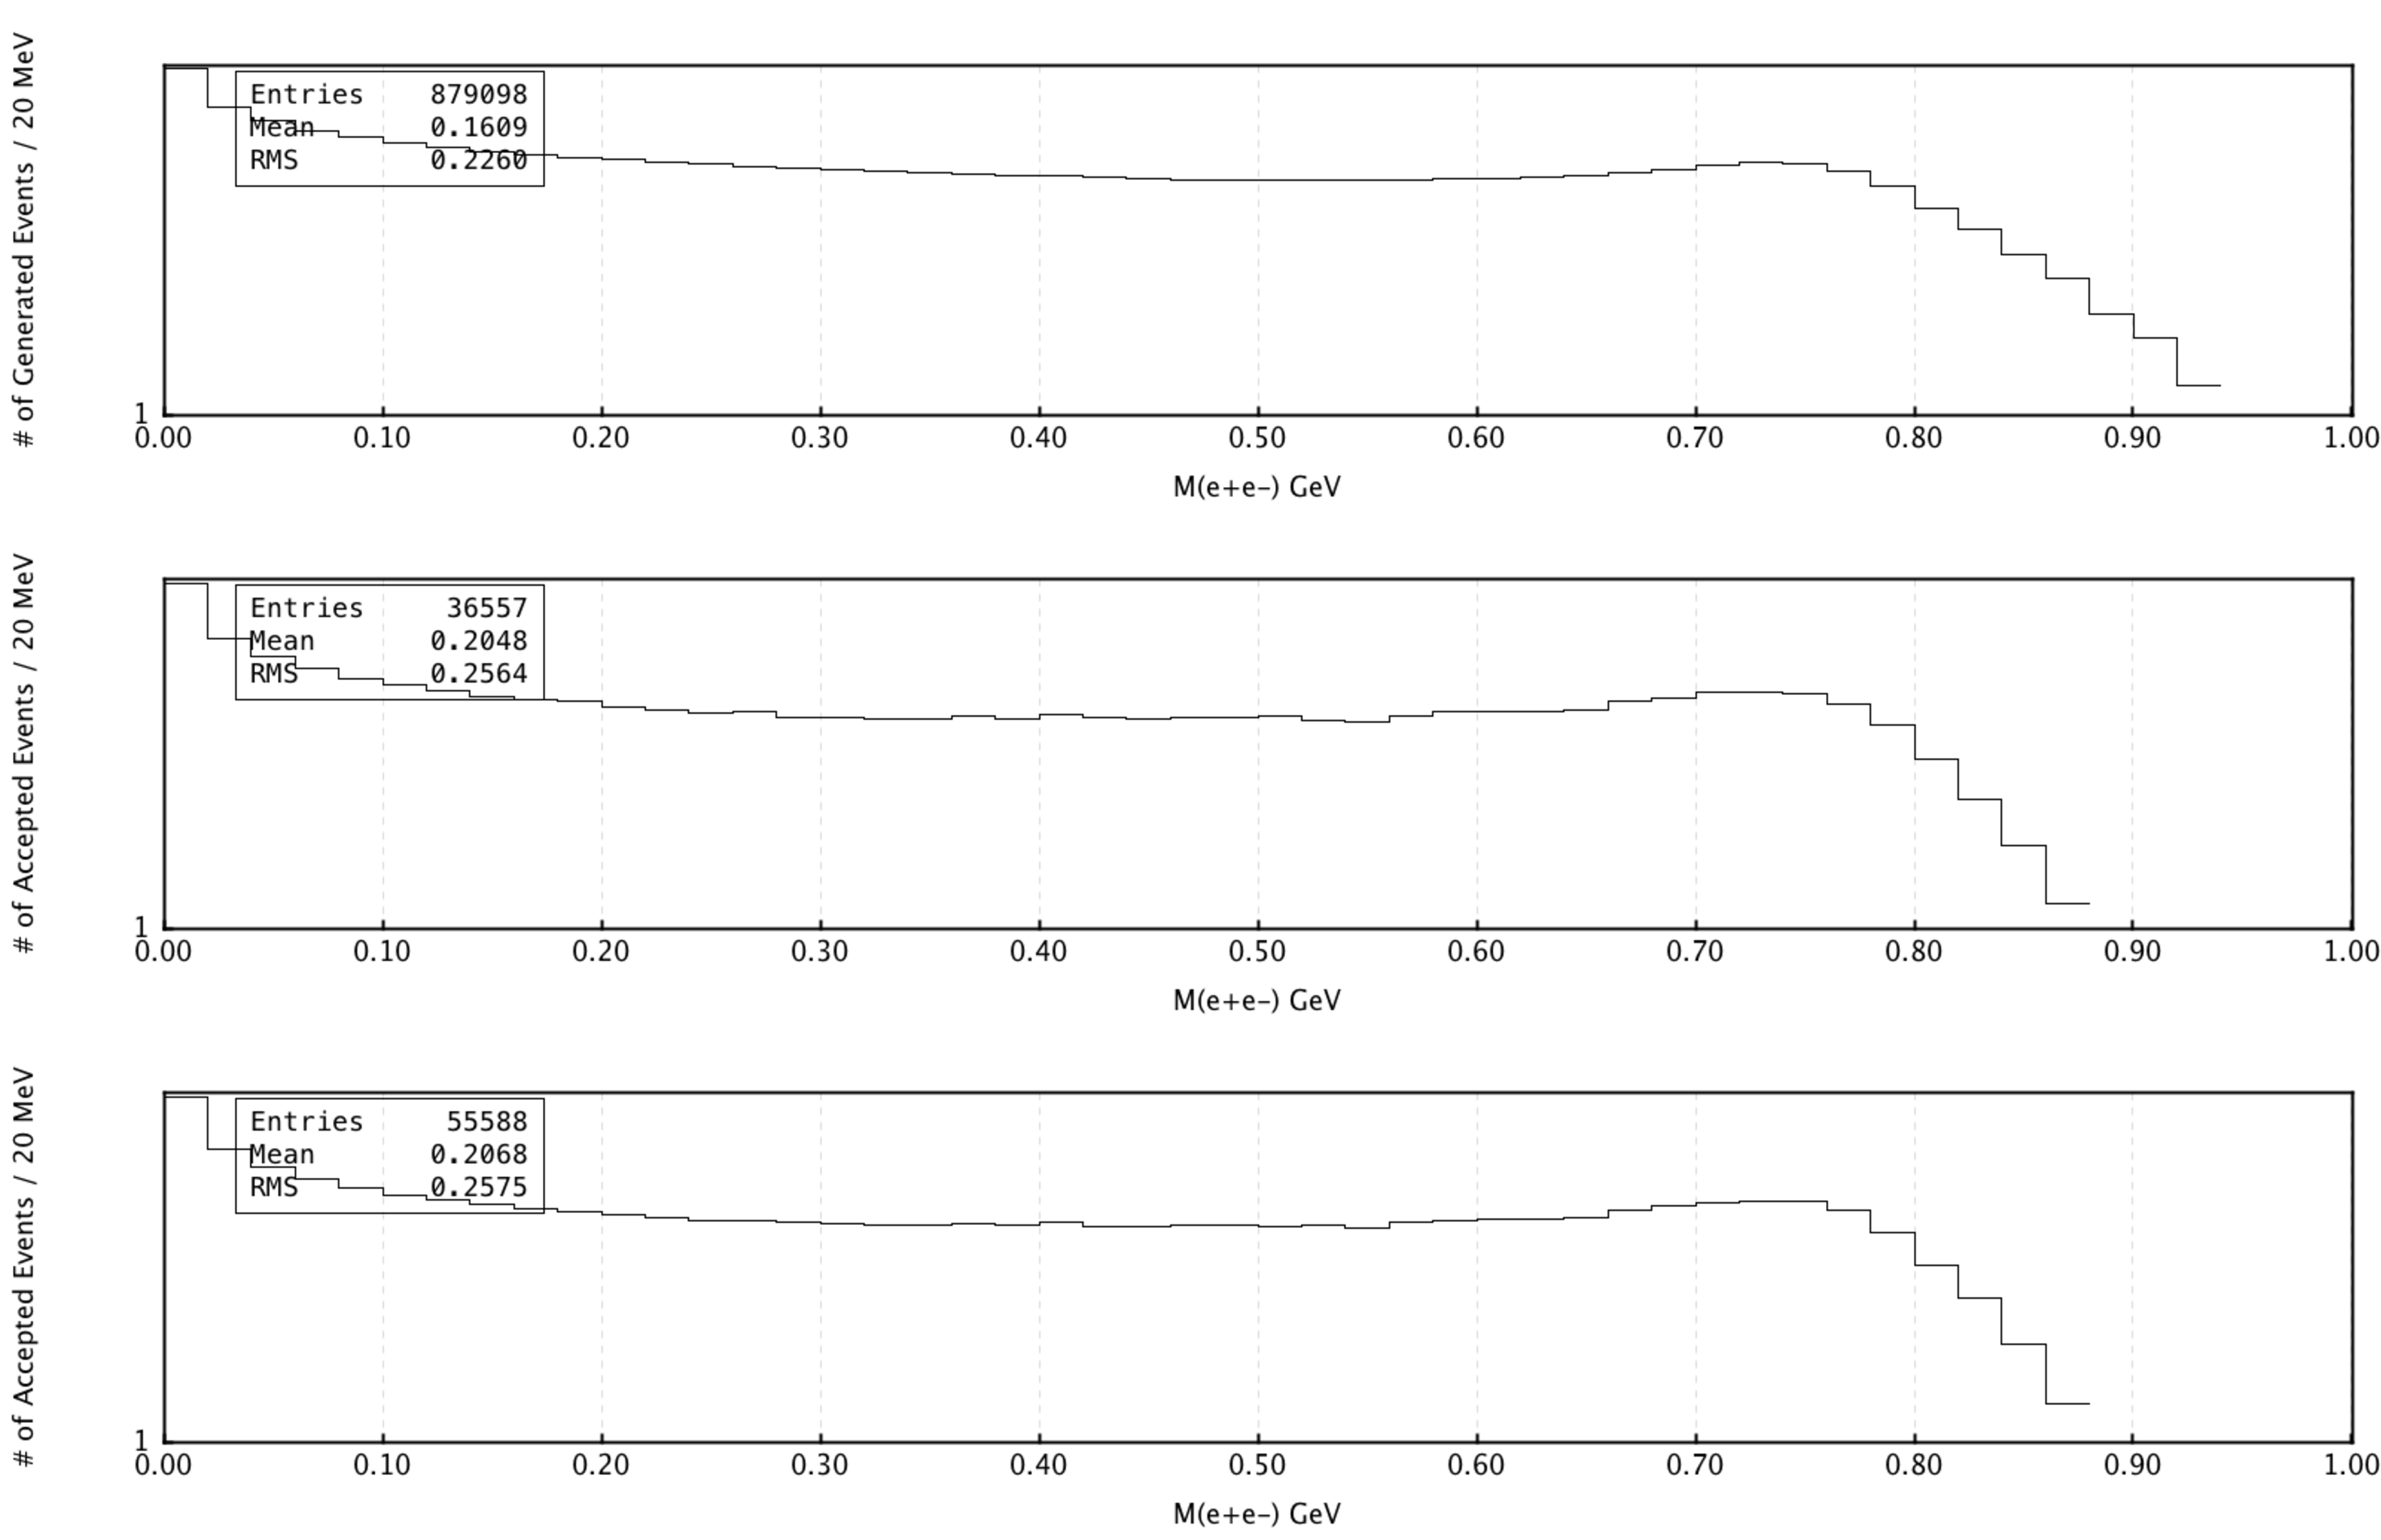
\includegraphics[width=\figwidth,height=2.6\qfigheight]{\grpath/counts/75_TORUS/VMD/VMD_Generated_Accepted.pdf}
%		\caption[Generated and Accepted counts, as a function of $M(\epem)$]{\label{fig:VMD}{Generated events (Top), accepted events for an exclusive (Middle), inclusive(Bottom) reconstruction schemes as a function of $M(\epem)$. In all panels a VMD decay model was employed}}
%\end{center}\end{figure}
%\begin{figure}[h!]\begin{center}
%			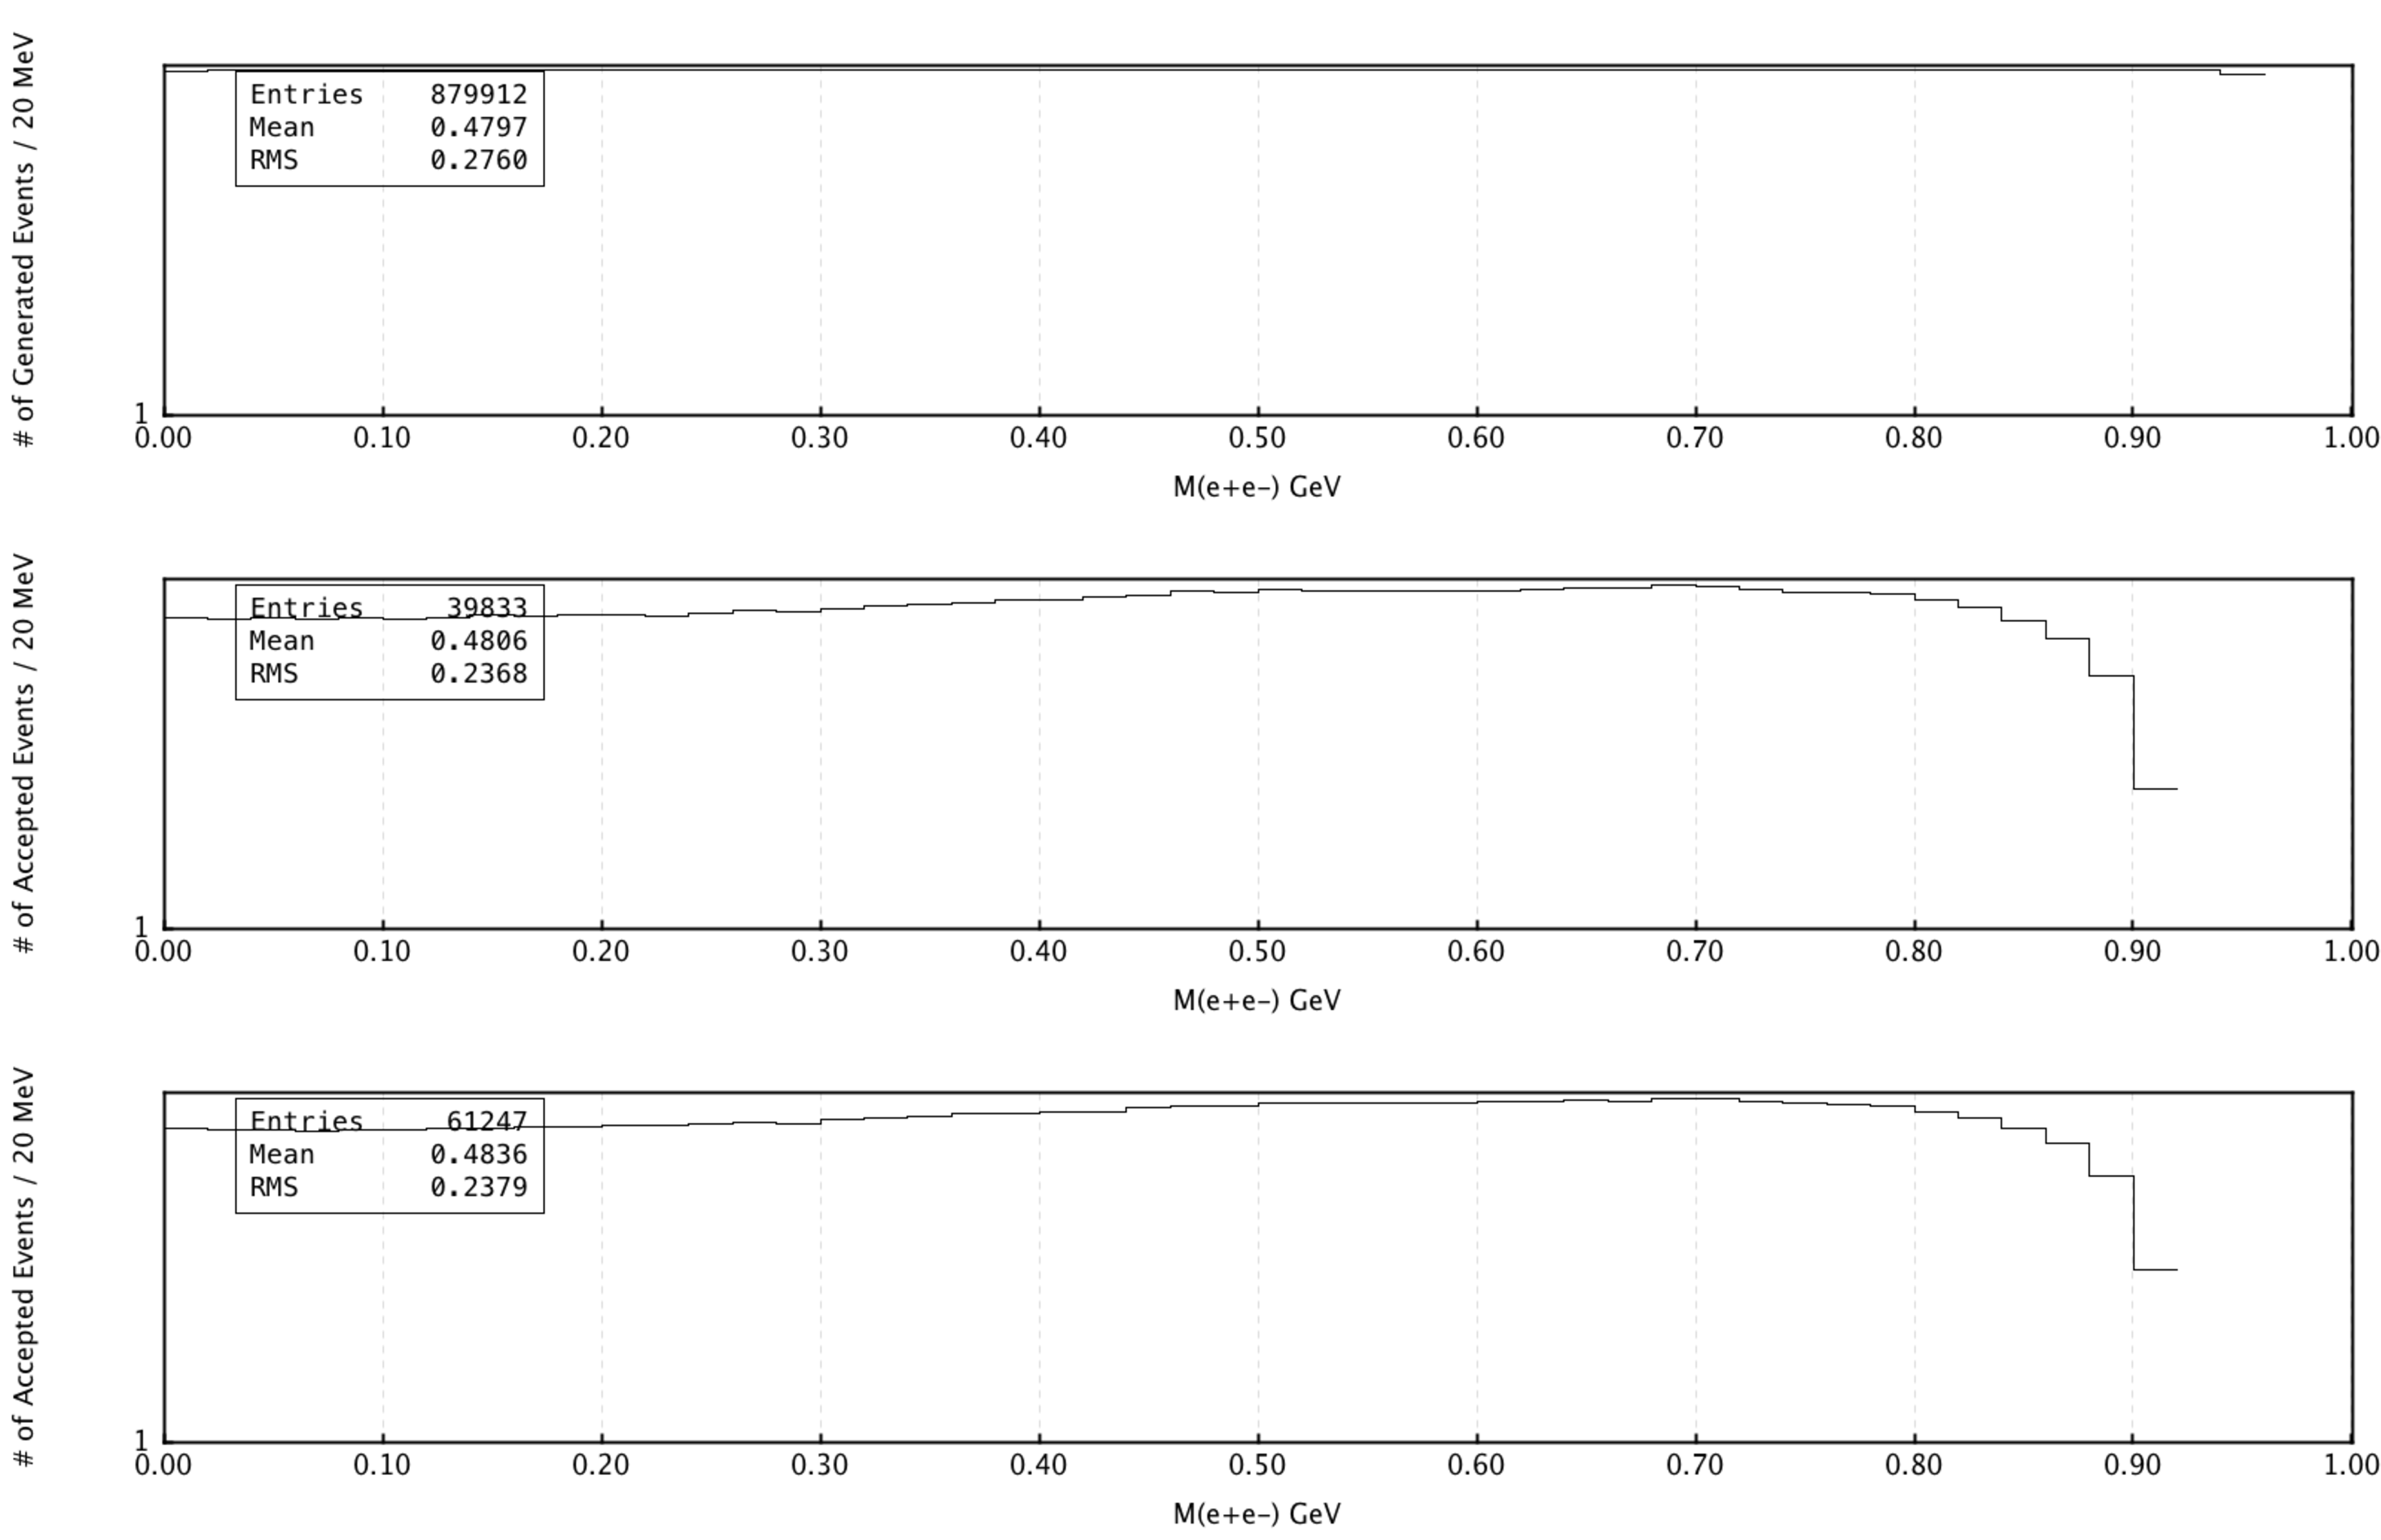
\includegraphics[width=\figwidth,height=2.6\qfigheight]{\grpath/counts/75_TORUS/FLAT/FLAT_Generated_Accepted.pdf}
%			\caption[Generated and Accepted counts, as a function of $M(\epem)$]{\label{fig:FLAT}{Generated events (Top), accepted events for an exclusive (Middle), inclusive(Bottom) reconstruction schemes as a function of $M(\epem)$. In all panels a Flat \epemT \ decay model was employed}}
%\end{center}\end{figure}
\FloatBarrier

\begin{figure}[h!]\begin{center}
		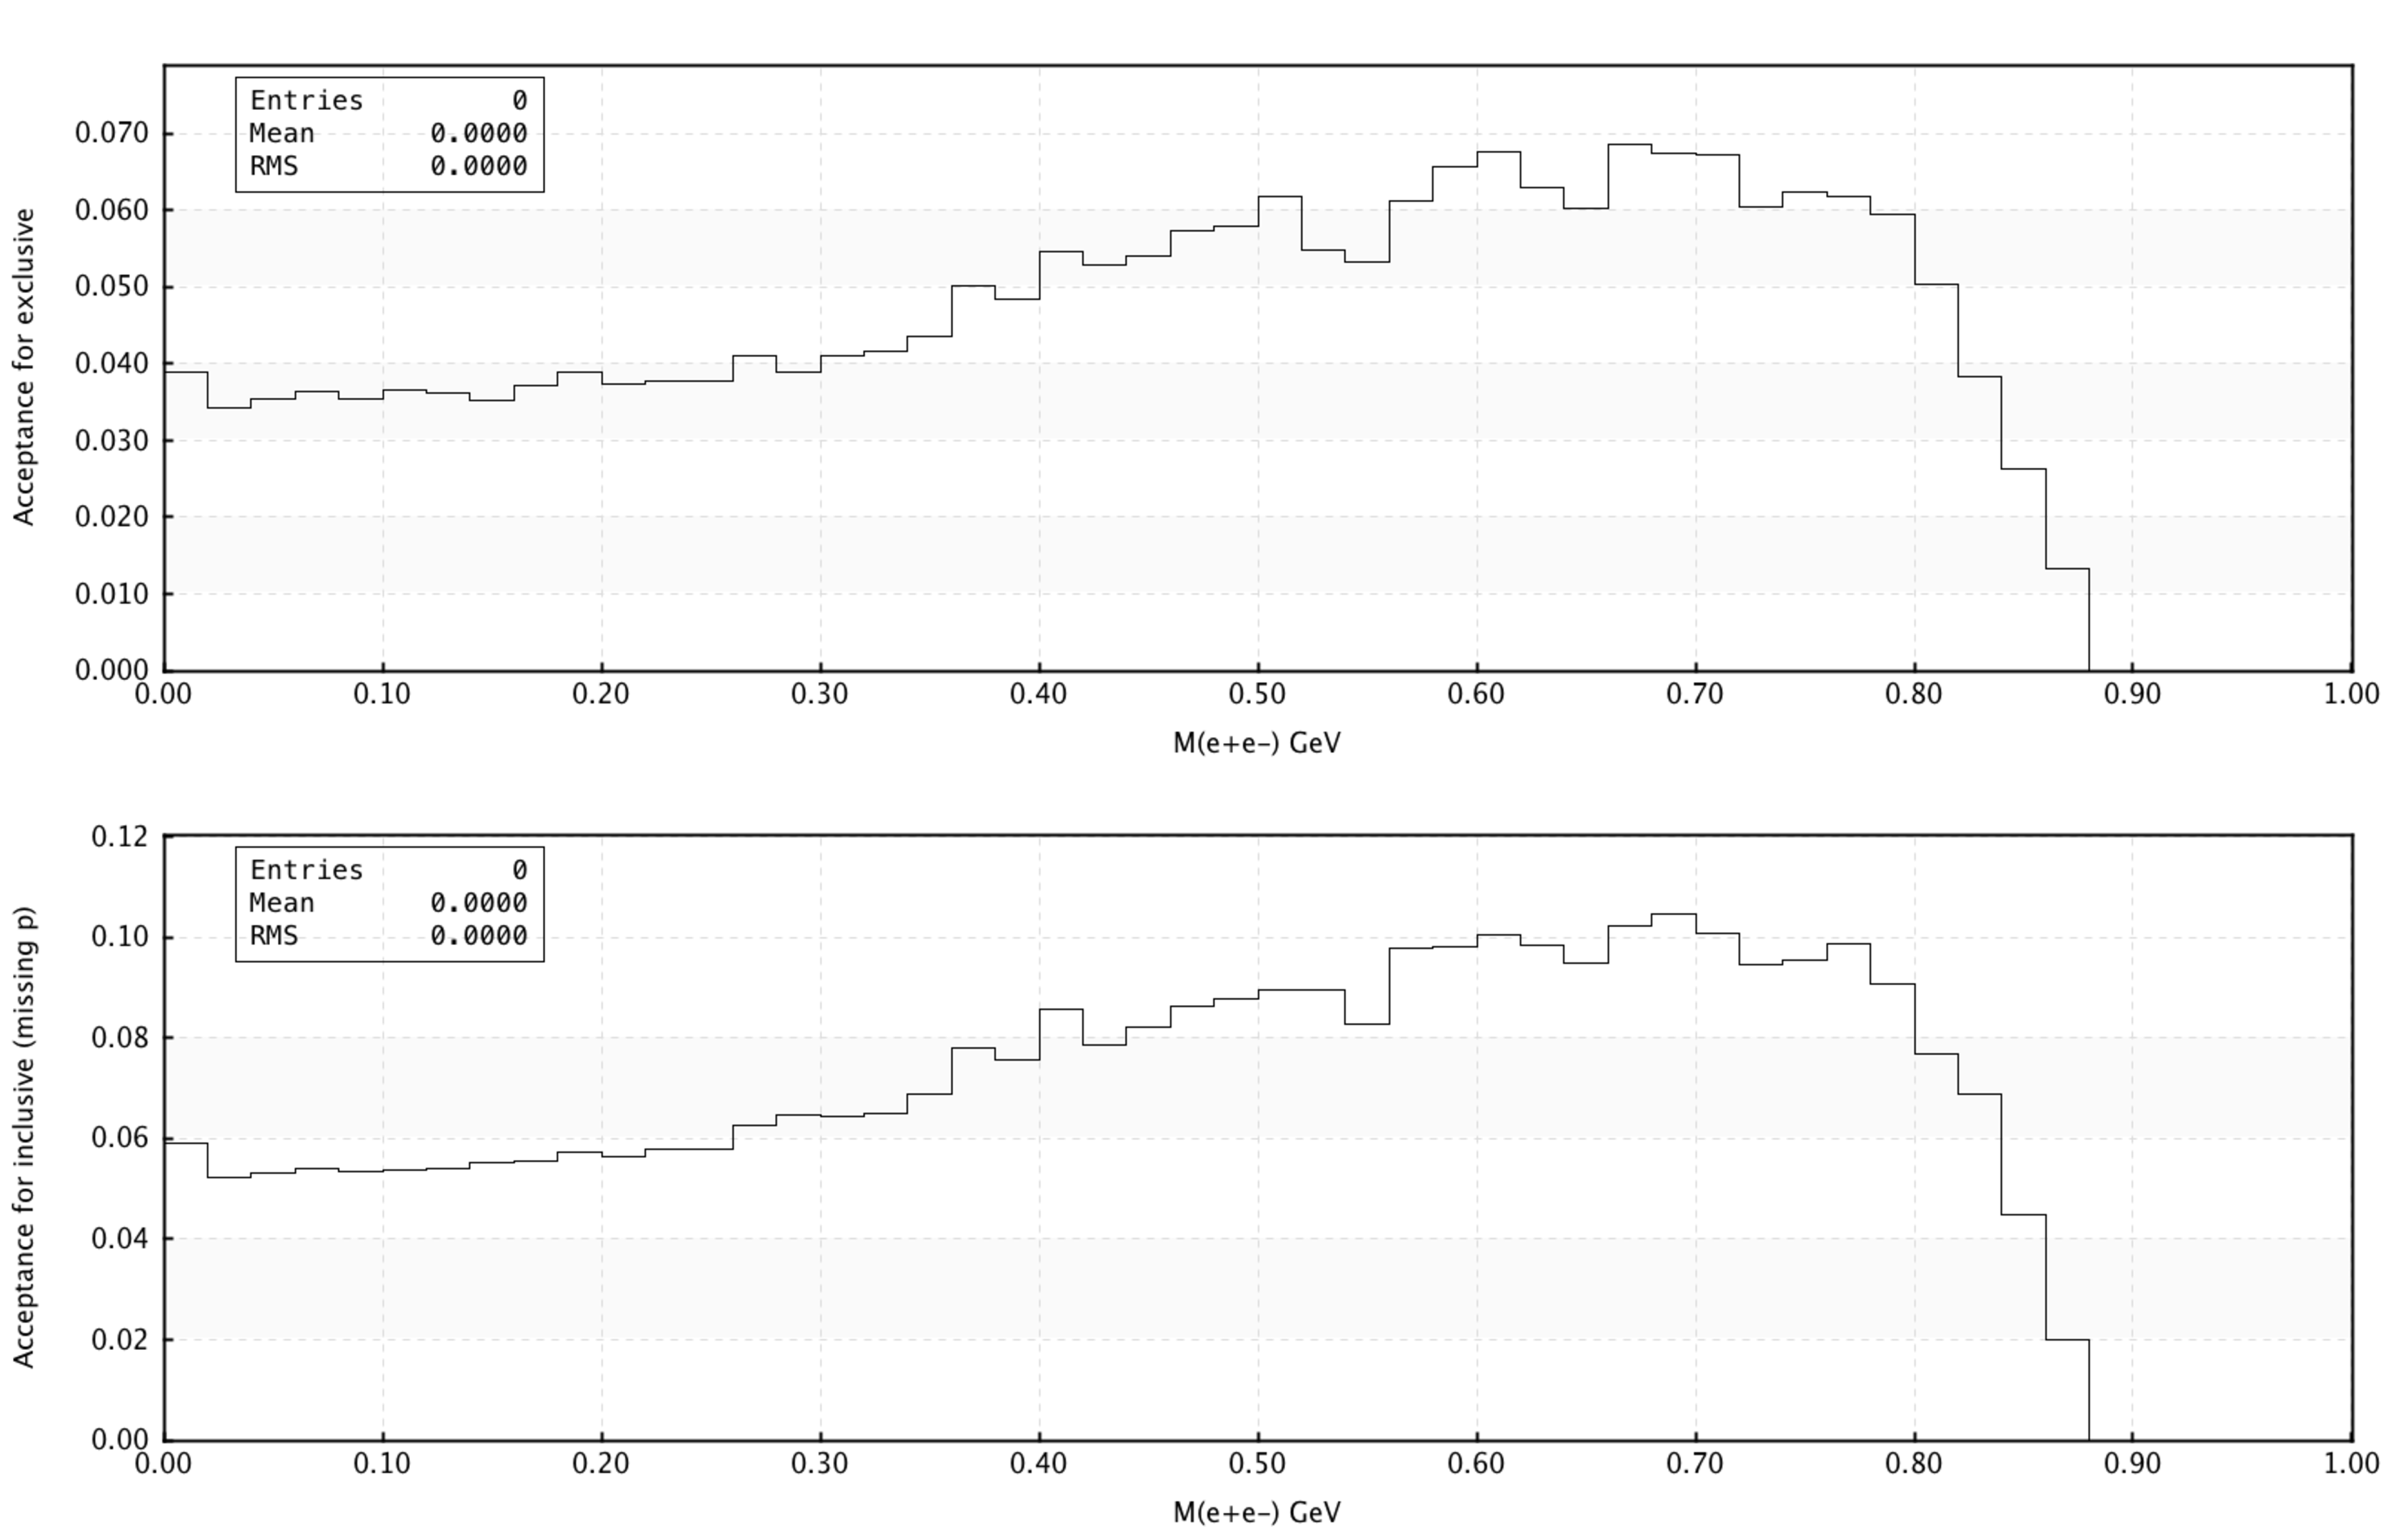
\includegraphics[width=\figwidth,height=1.2\qfigheight]{\grpath/counts/75_TORUS/VMD/VMD_Acceptance.pdf}
		\caption[Acceptance, as a function of $M(\epem)$]{\label{fig:VMDaccepted}{Acceptance using a VMD decay model, as a function of $M(\epem)$ for the exclusive (Top) and inclusive reconstruction scheme(Bottom). }}
\end{center}\end{figure}

 \begin{figure}[h!]\begin{center}
 		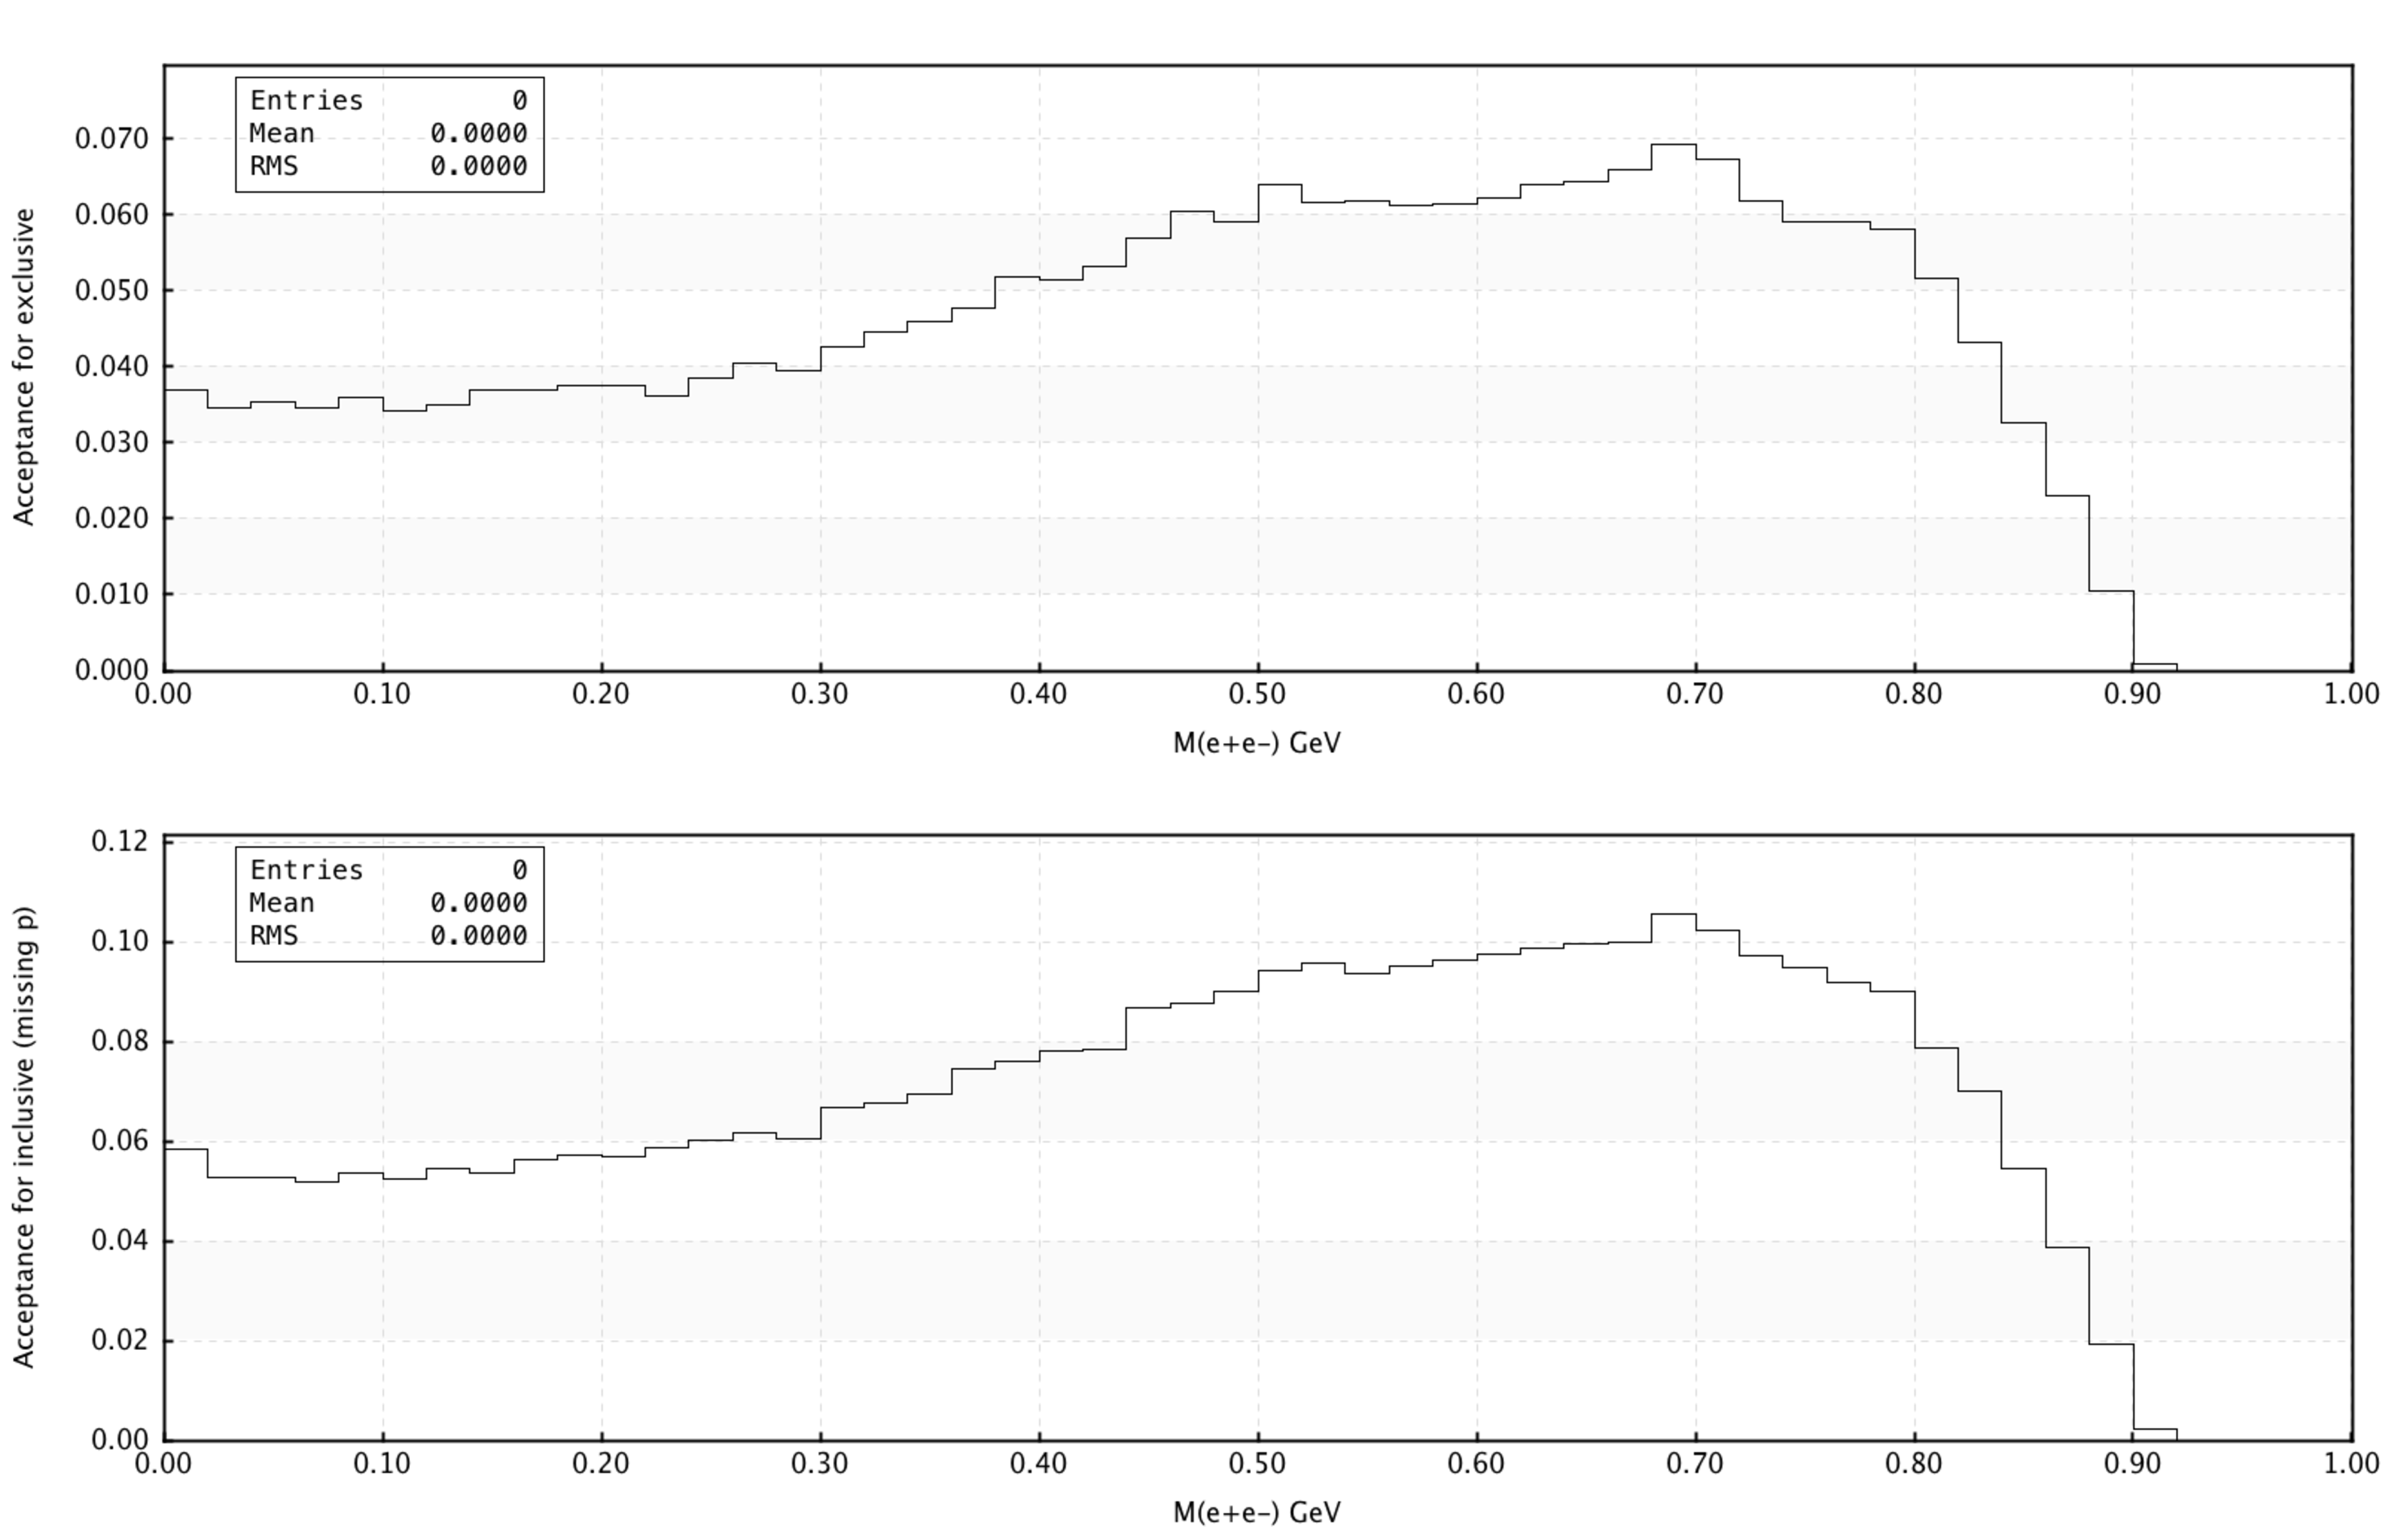
\includegraphics[width=\figwidth,height=1.2\qfigheight]{\grpath/counts/75_TORUS/FLAT/FLAT_Acceptance.pdf}
 		\caption[Acceptance, as a function of $M(\epem)$]{\label{fig:FLATaccepted}{Acceptance using a flat \epemT \ decay model, as a function of $M(\epem)$ for the exclusive (Top) and inclusive reconstruction scheme(Bottom).}}
 \end{center}\end{figure} 
\FloatBarrier




%%%%%%%%%%%%%%%%%%%%%%%%%%%%%%%%%%%%%%%
%THIS IS WHAT I ADDED:

\subsection{Calculating the Expected Yield}\label{sec:yield}
%\subsubsection{Calculating Photon Flux}\label{sec:calflux}
%A simple method for calculating the photon flux in CLAS12 is as follows; Using the fact that g12 had a photon flux of $7\cdot 10^7 \ \mathrm{\gamma/s}$ on a Au radiator of $10^{-4} \chi_0$ an expected $\sim 4\cdot 10^9  \mathrm{\gamma/s}$ will be seen in CLAS12 at ${\cal L} = 10^{35}\mathrm{cm^{-2}s^{-1}}$ on a 5~cm $\ell H_2$ target which is $\sim 5.7\cdot 10^{-3} \chi_0$. This number has been independently confirmed in a previous CLAS proposal~\cite{clas.proposal.meson}.

The expected yield for $ep\to e'p \etaP [\etaP\rightarrow p e^+e^- \gamma ]$ is calculated under the assumption, that the $\etaP$ electro-production cross-section can be deduced from the $\etaP$ photo-production cross-section. A qualitative justification of this assumption may be found in Fig.~\ref{fig:EtaProdX}. The shape of the cross-section distributions for $ep\rightarrow e'p\eta$, shown in the top row of Fig.~\ref{fig:EtaProdX}, are comparable to the corresponding distribution for $\gamma p\rightarrow p\eta$, plotted in the bottom row of Fig.~\ref{fig:EtaProdX}. The major difference is related to the scaling rule of $1/Q^2$, i.e. the electro-production cross-section might be approximated by the photo-production cross-section by scaling down the latter one by $1/Q^2$.

\begin{figure}[htbp]\begin{center}
		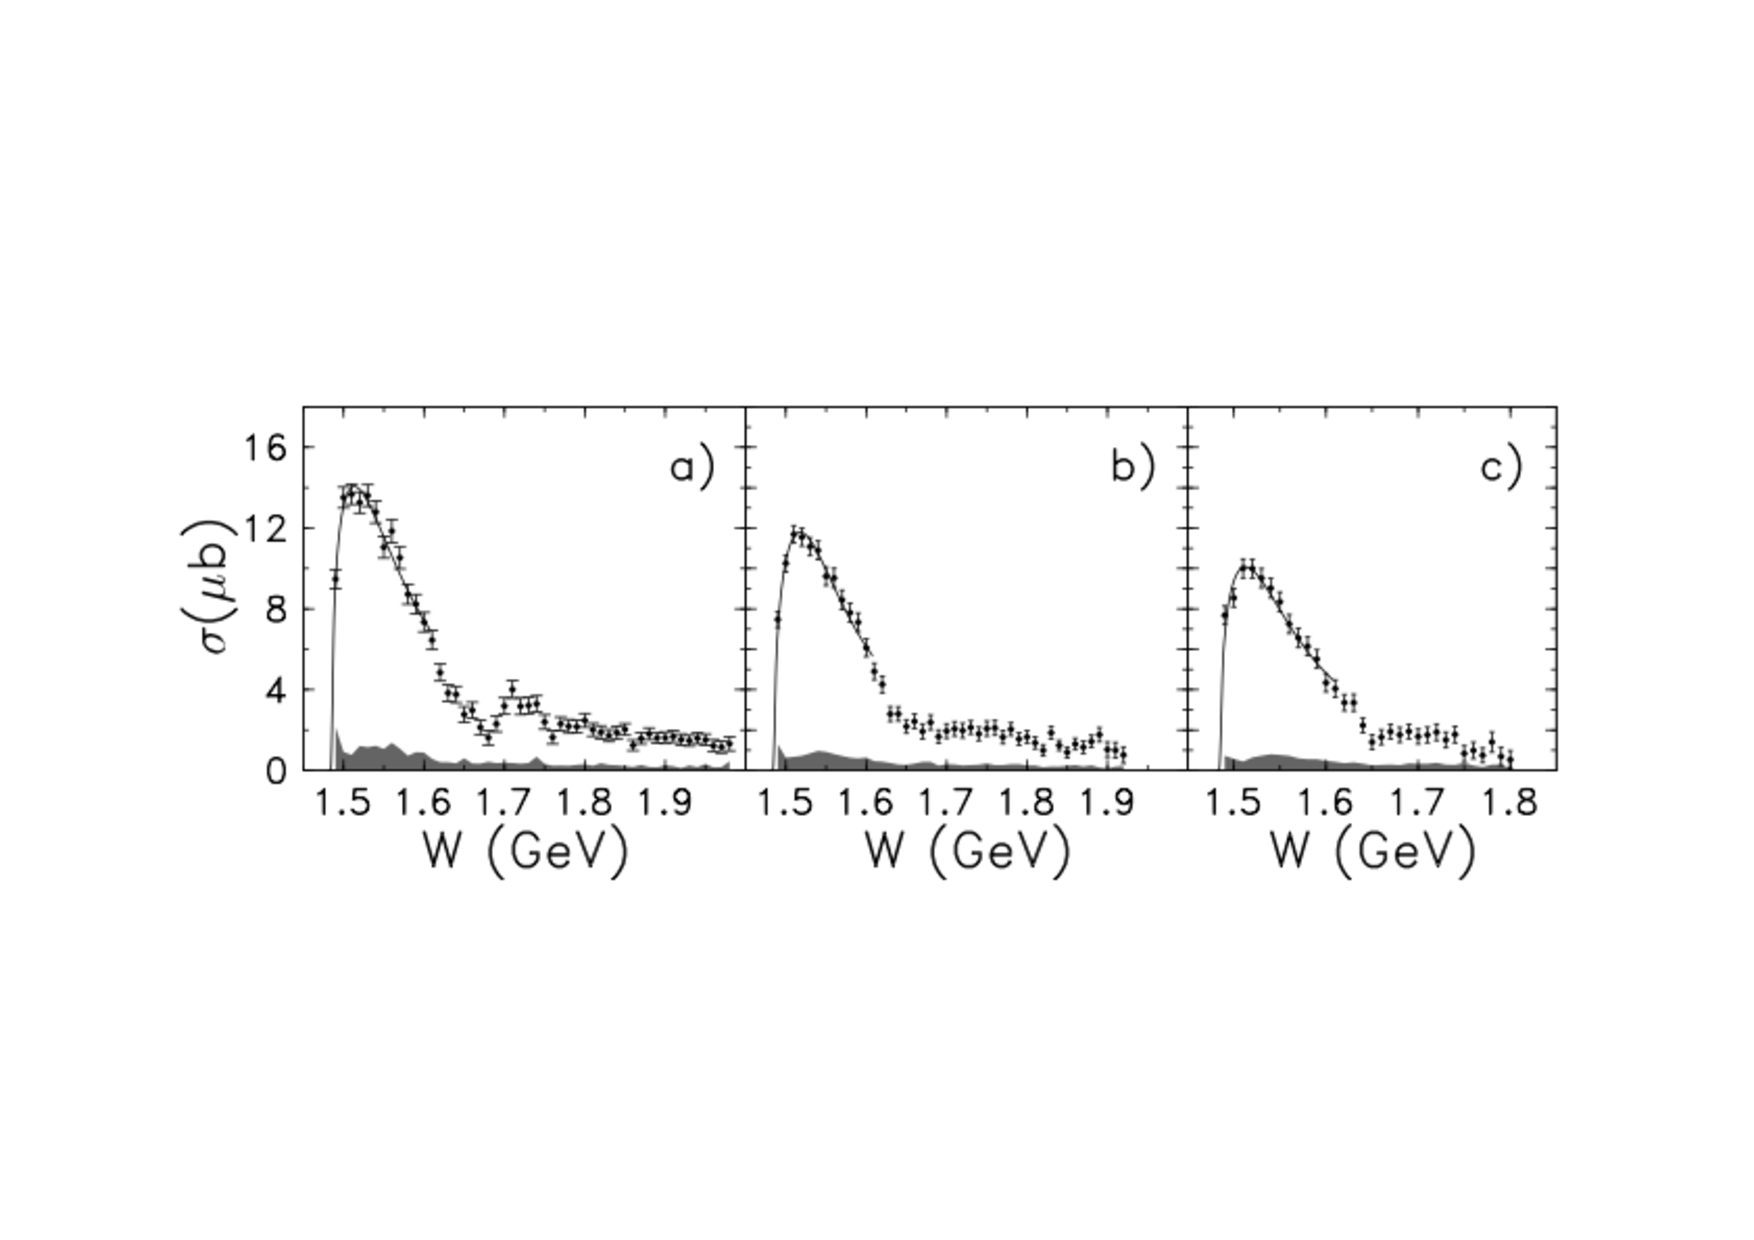
\includegraphics[width=\figwidth,height=1.2\qfigheight]{\grpath/XSection/eta_phot_electXSection.pdf}\\
		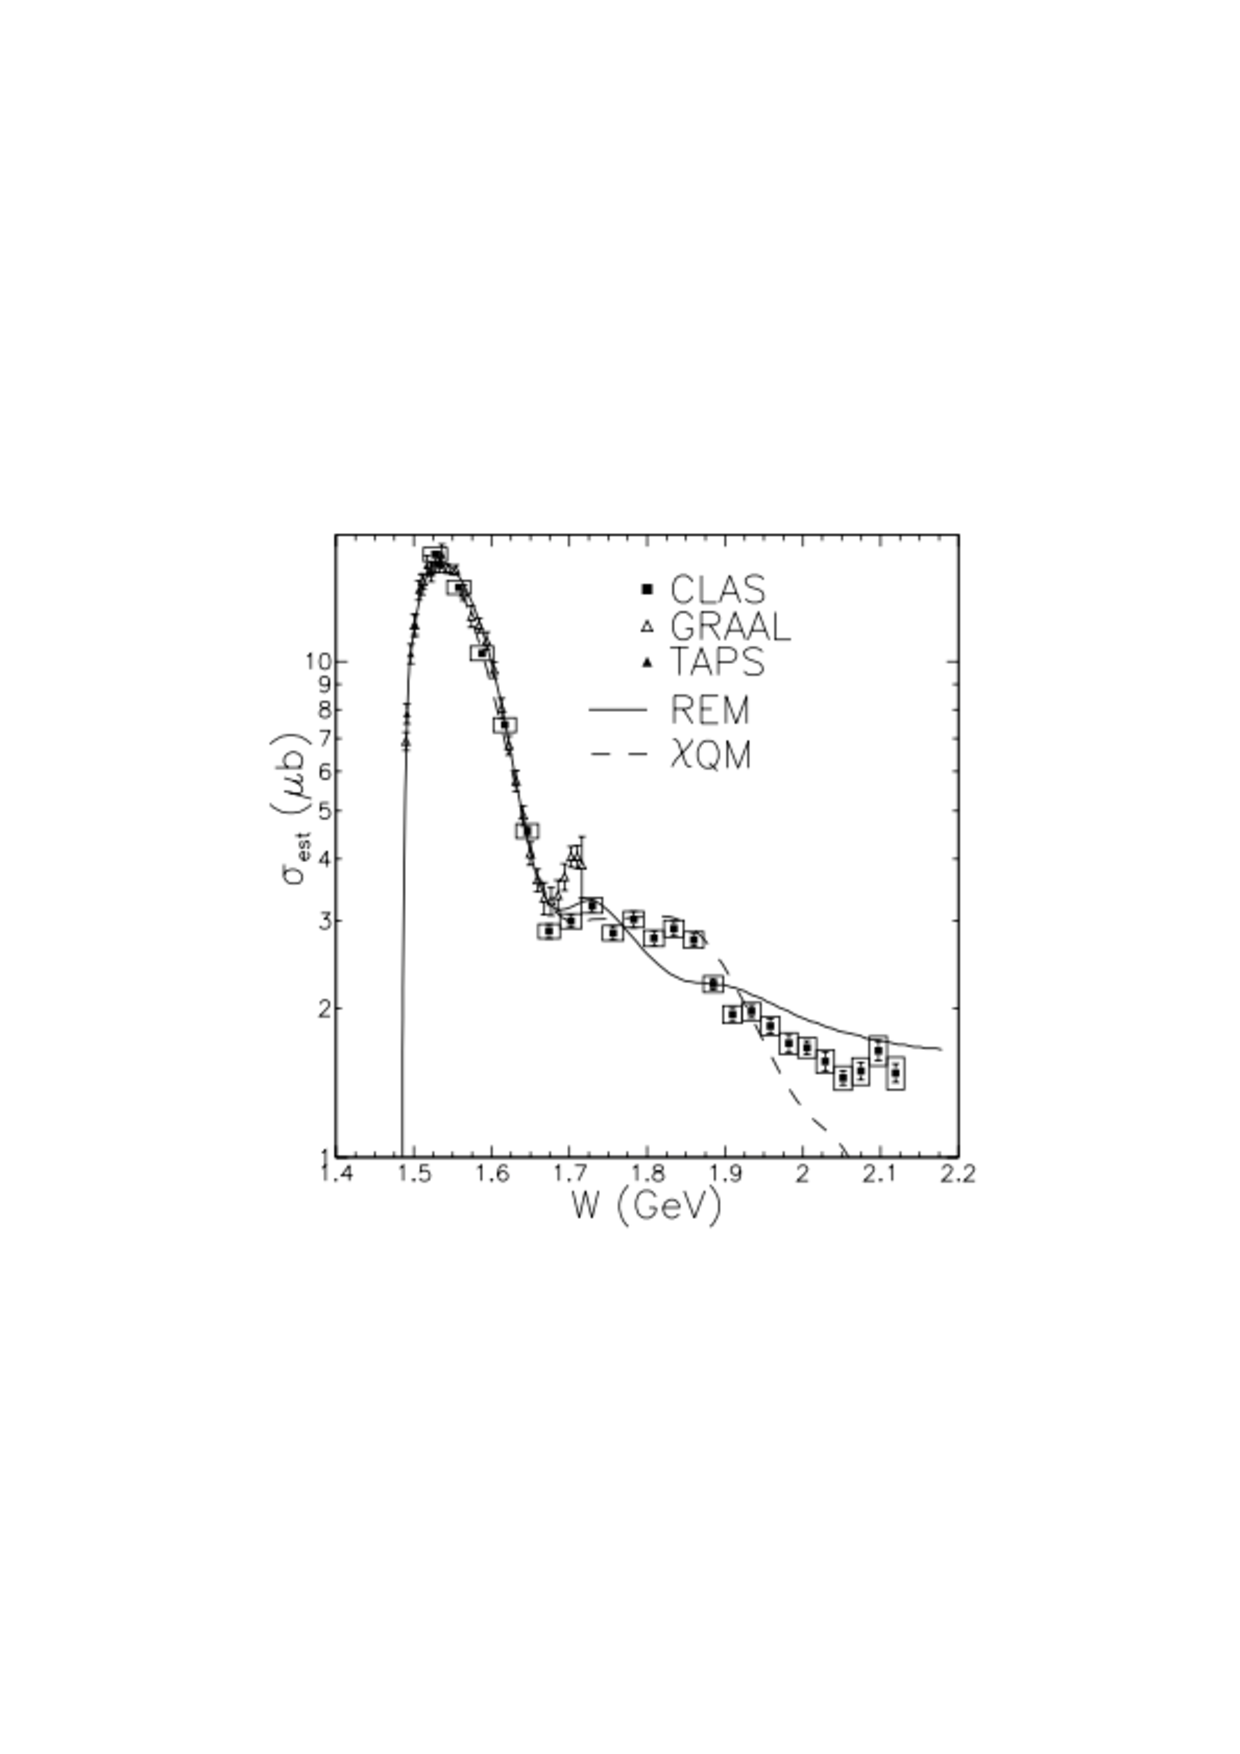
\includegraphics[width=0.7\figwidth,height=0.9\qfigheight]{\grpath/XSection/eta_phot_prodXSection.pdf}
		\caption[eta el-prod. XSection]{\label{fig:EtaProdX}{Integrated cross-section for $ep\to e'p\eta$ (Top) for: (a) $Q^2=0.625(GeV/c)^2$, (b) $Q^2=0.875(GeV/c)^2$, (a) $Q^2=1.125(GeV/c)^2$~\cite{etaelect} and for $\gamma p\rightarrow p\eta$ (Bottom)~\cite{etaphoto}.}}
\end{center}\end{figure}

\FloatBarrier

The top row of Fig.~\ref{fig:EtaPProdX} shows the total photo-production cross-section for hadrons in comparison with the photo-production cross-section for $\etaP$ (see bottom row of Fig.~\ref{fig:EtaPProdX}). Due to the considerations made above, these two cross-section distributions might be directly translated to the corresponding electro-production cross-sections. Using the distributions shown in Fig.~\ref{fig:EtaPProdX}, one might define the following ratio $R(W)$:

\begin{equation}
 R(W) = \frac{\sigma(W)}{\etaP\text{ integrated } \sigma(W)}
\label{XsecR}
\end{equation}

\begin{figure}[h!]\begin{center}
		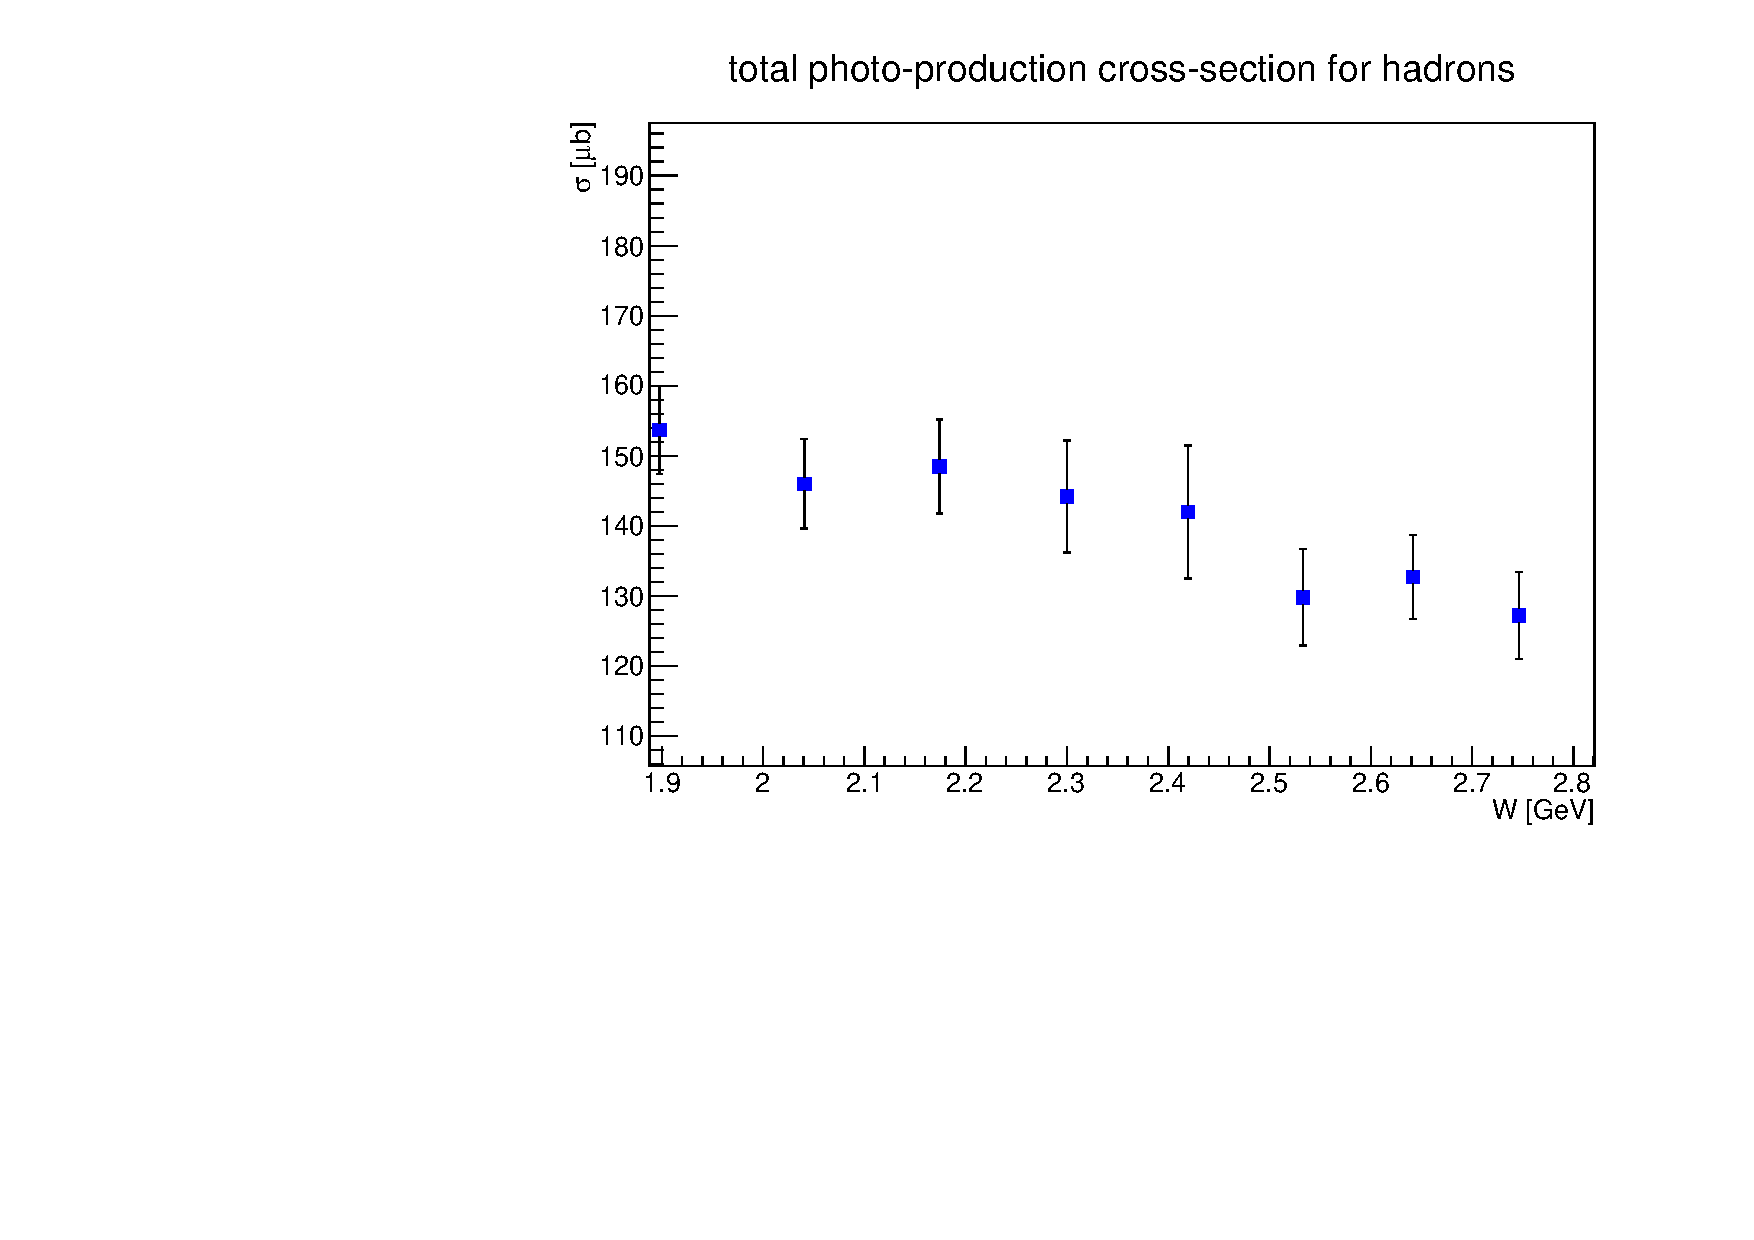
\includegraphics[width=0.9\figwidth,height=0.9\qfigheight]{\grpath/XSection/hadron_prod_photoproduction.pdf}\\
		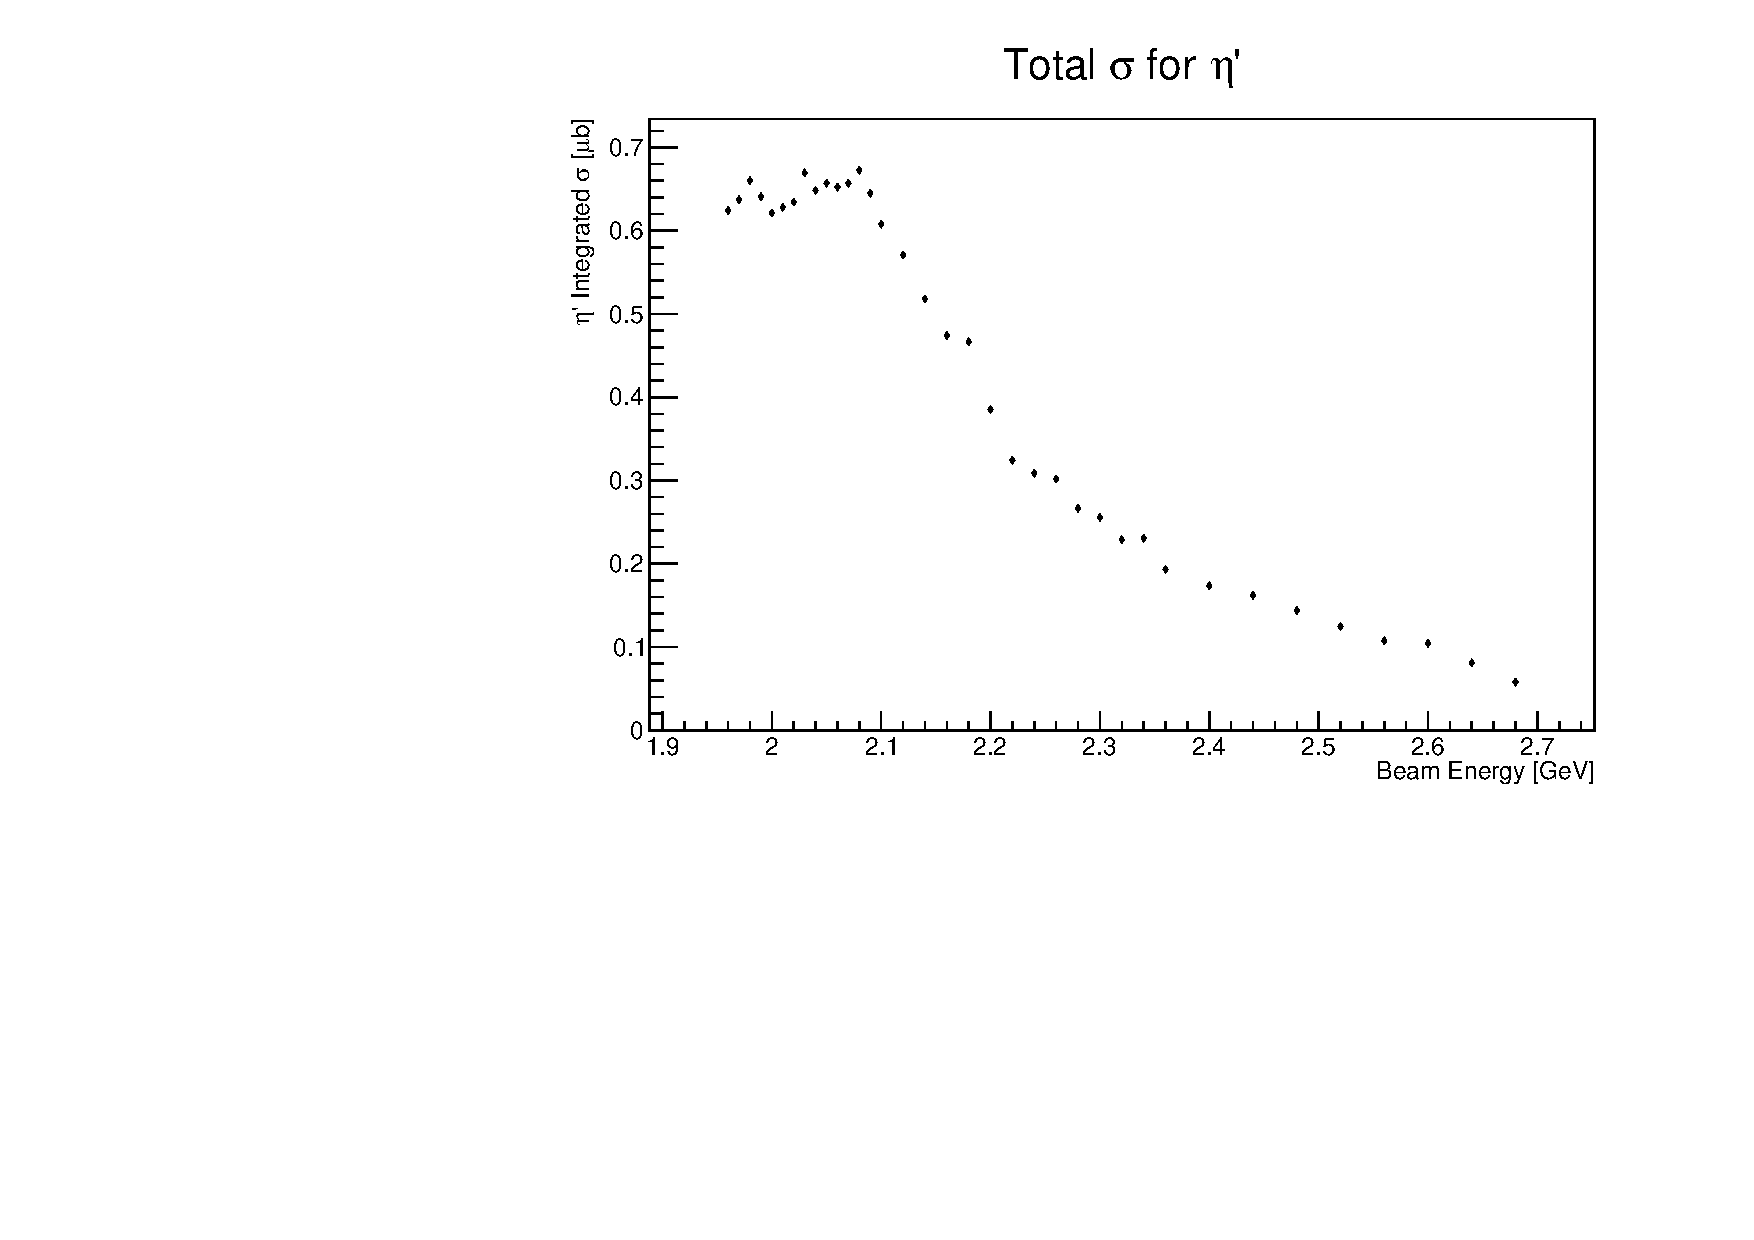
\includegraphics[width=0.9\figwidth,height=0.9\qfigheight]{\grpath/XSection/etaP_total_XSection.pdf}
		\caption[etaP phot-prod. XSection]{\label{fig:EtaPProdX}{Integrated cross-section for $\gamma p\rightarrow pX$ (Top) and $\gamma p\rightarrow p\etaP$ (Bottom) as a function of $W$.}}
\end{center}\end{figure}

The rate for mesons in electro-production where the scattered electron is left undetected is $\sim 140\,\rm{kHz}$~\cite{Sargsyan}. This rate needs to be scaled down by $R(W)$ in order to achieve the corresponding rate for $\etaP$ production. This leads to:

\begin{equation}
 \etaP\text{ total rates / 80 Days }(W) = 140\,\rm{kHz}\cdot \frac{86,400\mathrm{\ seconds}}{\text{80 days}}\cdot \frac{1}{R(W)}
\label{etaPRate}
\end{equation}

A plot of Eq.~\ref{etaPRate} is shown in Fig.~\ref{fig:EtaPRate} (left y-axis). The total $\etaP\rightarrow\epem\gamma$ rates per 80 days, and as a function $W$, is calculated by multiplying Eq.\ref{etaPRate} with the product of the average detection efficiency $\epsilon\approx 5\%$ as well as the branching fraction $\mathcal{BR} $ for $\etaP\rightarrow\epem\gamma$. The corresponding plot is shown in Fig.~\ref{fig:EtaPRate} (right y-axis). Obviously, the total number $N_{tot}$ of expected $\etaP\rightarrow\epem\gamma$ events after 80 days of measurement is given by the integral of Fig.~\ref{fig:EtaPRate} over $W$. This leads to the expected yield:

\begin{equation}
  N_{tot} = \int\limits_{1.9\,\rm{GeV}}^{2.8\,\rm{GeV}} \Big[ {\color{red}{N(W)_{\etaP\rightarrow\epem\gamma\text{ / 80 Days }}}} \Big]dW = \mathrm{\frac{52,100 \ events}{80 Days}}
\label{yield}
\end{equation}


\begin{figure}[h!]\begin{center}
		\includegraphics[width=0.9\figwidth,height=0.9\qfigheight]{\grpath/XSection/Total_rates.pdf}\\
		\caption[etaP rates]{\label{fig:EtaPRate}{Total $\etaP$ production rate per 80 days (left y-axis) and total $\etaP\rightarrow \epem\gamma$ rates per 80 days (right y-axis) as a function of $W$. Both rates have been calculated according to Eq.~\ref{etaPRate}}}
\end{center}\end{figure}


%%%%%%%%%%%%%%%%%%%%%%%%%%%%%%%%%%%%%%%





%\subsubsection{Expected Results}
%To extrapolate the number of $\etaP$ \ produced in 
%\\
%The average number of $\mathrm{meson} \to \epem X$ expected in CLAS12 can be calculated as:
%\begin{align}
%\bar{N}(\epem)_{\mathrm{meson}  \to \epem X} = \Phi \epsilon(\epem)\bar{\sigma} \rho_{\ell_{H_2}}\ell_{target}N_A \frac{\Gamma_{\mathrm{tot}_\mathrm{meson} }}{\Gamma_{\mathrm{meson}  \to \epem X}}\ ,
%\end{align}
%where $\Phi$ is the photon flux estimated in Sec.~\ref{sec:calflux}, $\epsilon$ is the acceptance, $\bar{\sigma}$ is the total cross-section, $\rho_{\ell_{H_2}}$ is the atomic density of $\ell_{H_2}$, $\ell_{target}$ is the target length, $N_A$ is Avogadro's constant, and $\frac{\Gamma_{\mathrm{tot}_\mathrm{meson}}}{\Gamma_{\mathrm{meson} \to \epem X}}$ is the total branching fraction of the meson decaying into $\epem X$.
%Using the lepton acceptance shown is Sec.~\ref{sec.reconstruction} the average number of \etaTP \  per $M(\epem)$ can be seen in Fig.~\ref{fig:etayield}.
% \begin{figure}[h!]\begin{center}
% \subfloat[$\etaP$ Dalitz and conversion spectra][]{ %Feynman diagram of $\etaP$ two photon decay
%	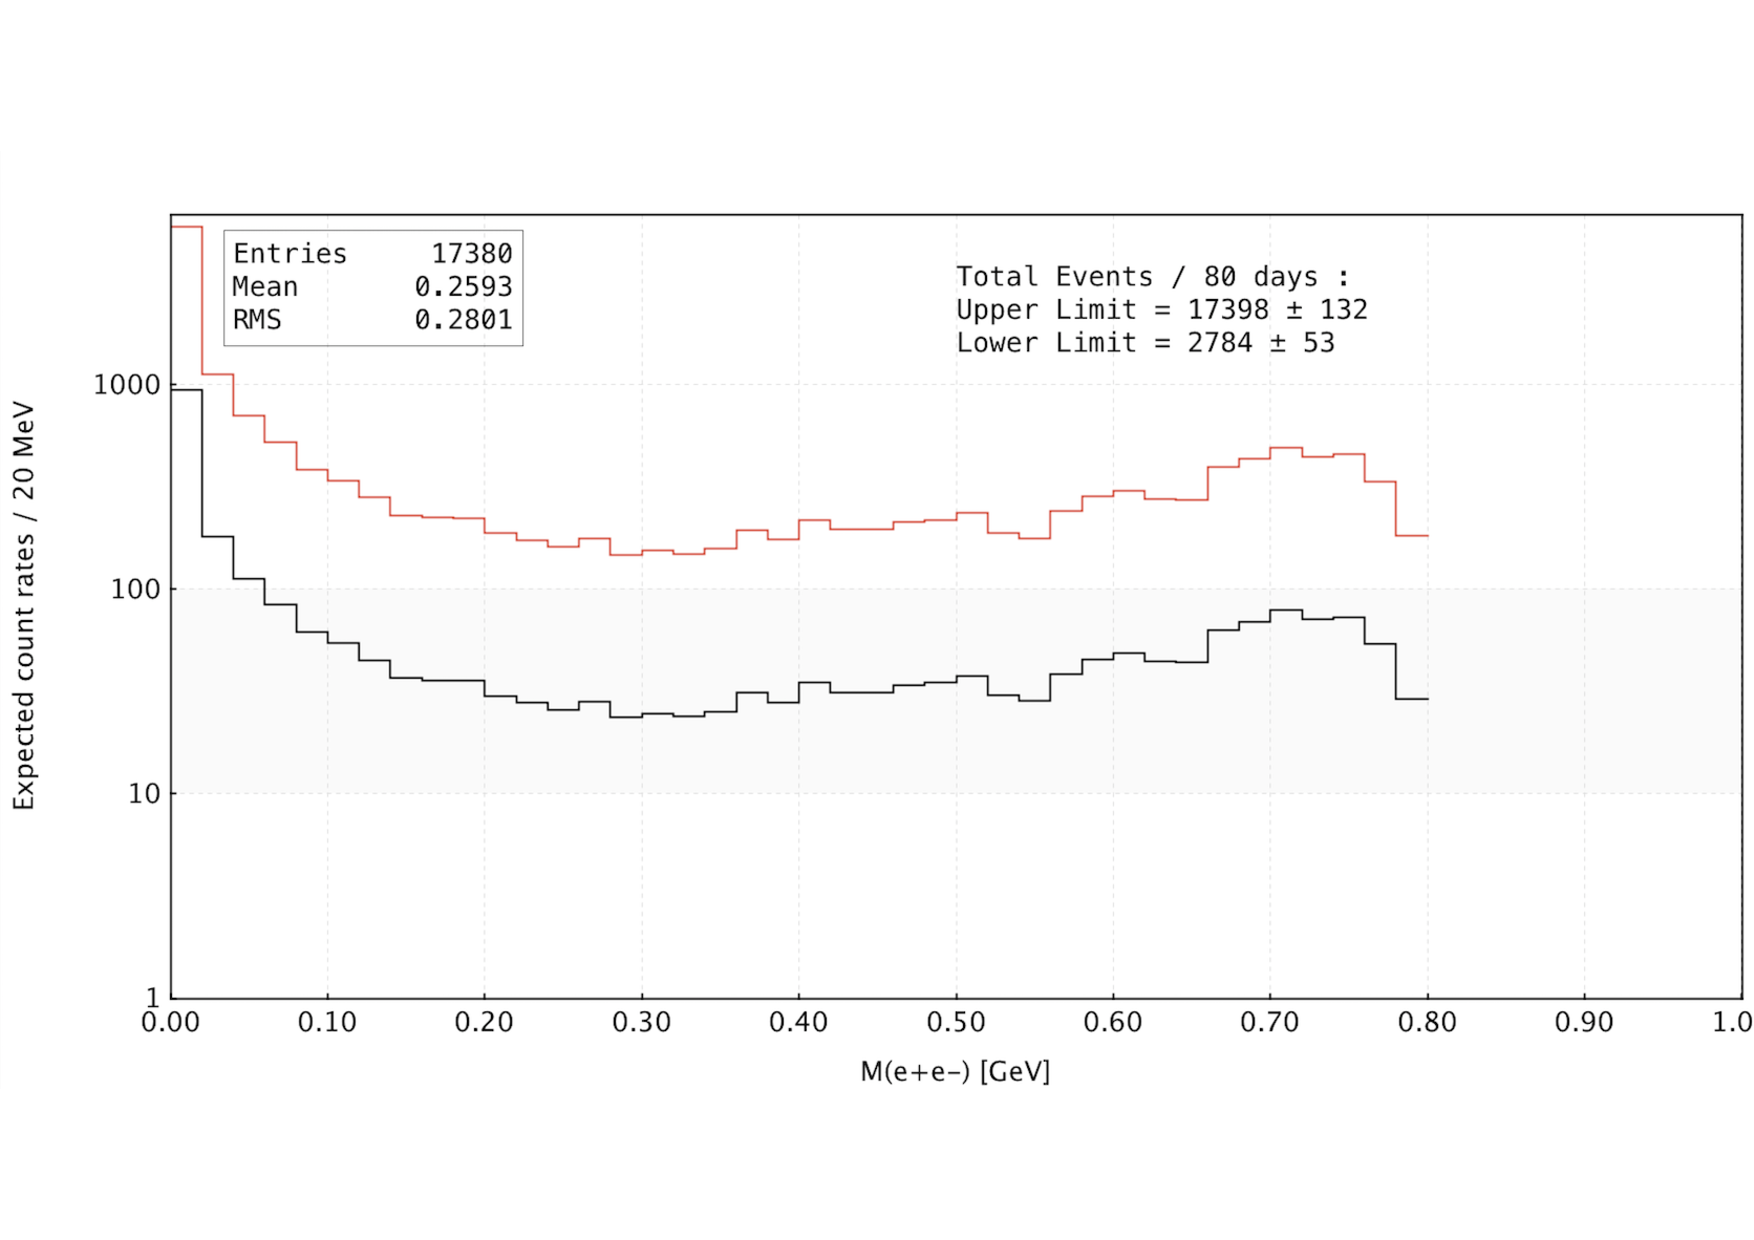
\includegraphics[width=0.8\columnwidth,height=1.0\qfigheight]{\grpath/counts/75_TORUS/VMD/VMD_Excluvise_count_rate.pdf}\label{fig:etap_count_exclu}
%	}
%\\
%\subfloat[$\phi$ Dalitz and conversion spectra][]{ %Feynman diagram of $\etaP$ Dalitz decay
%	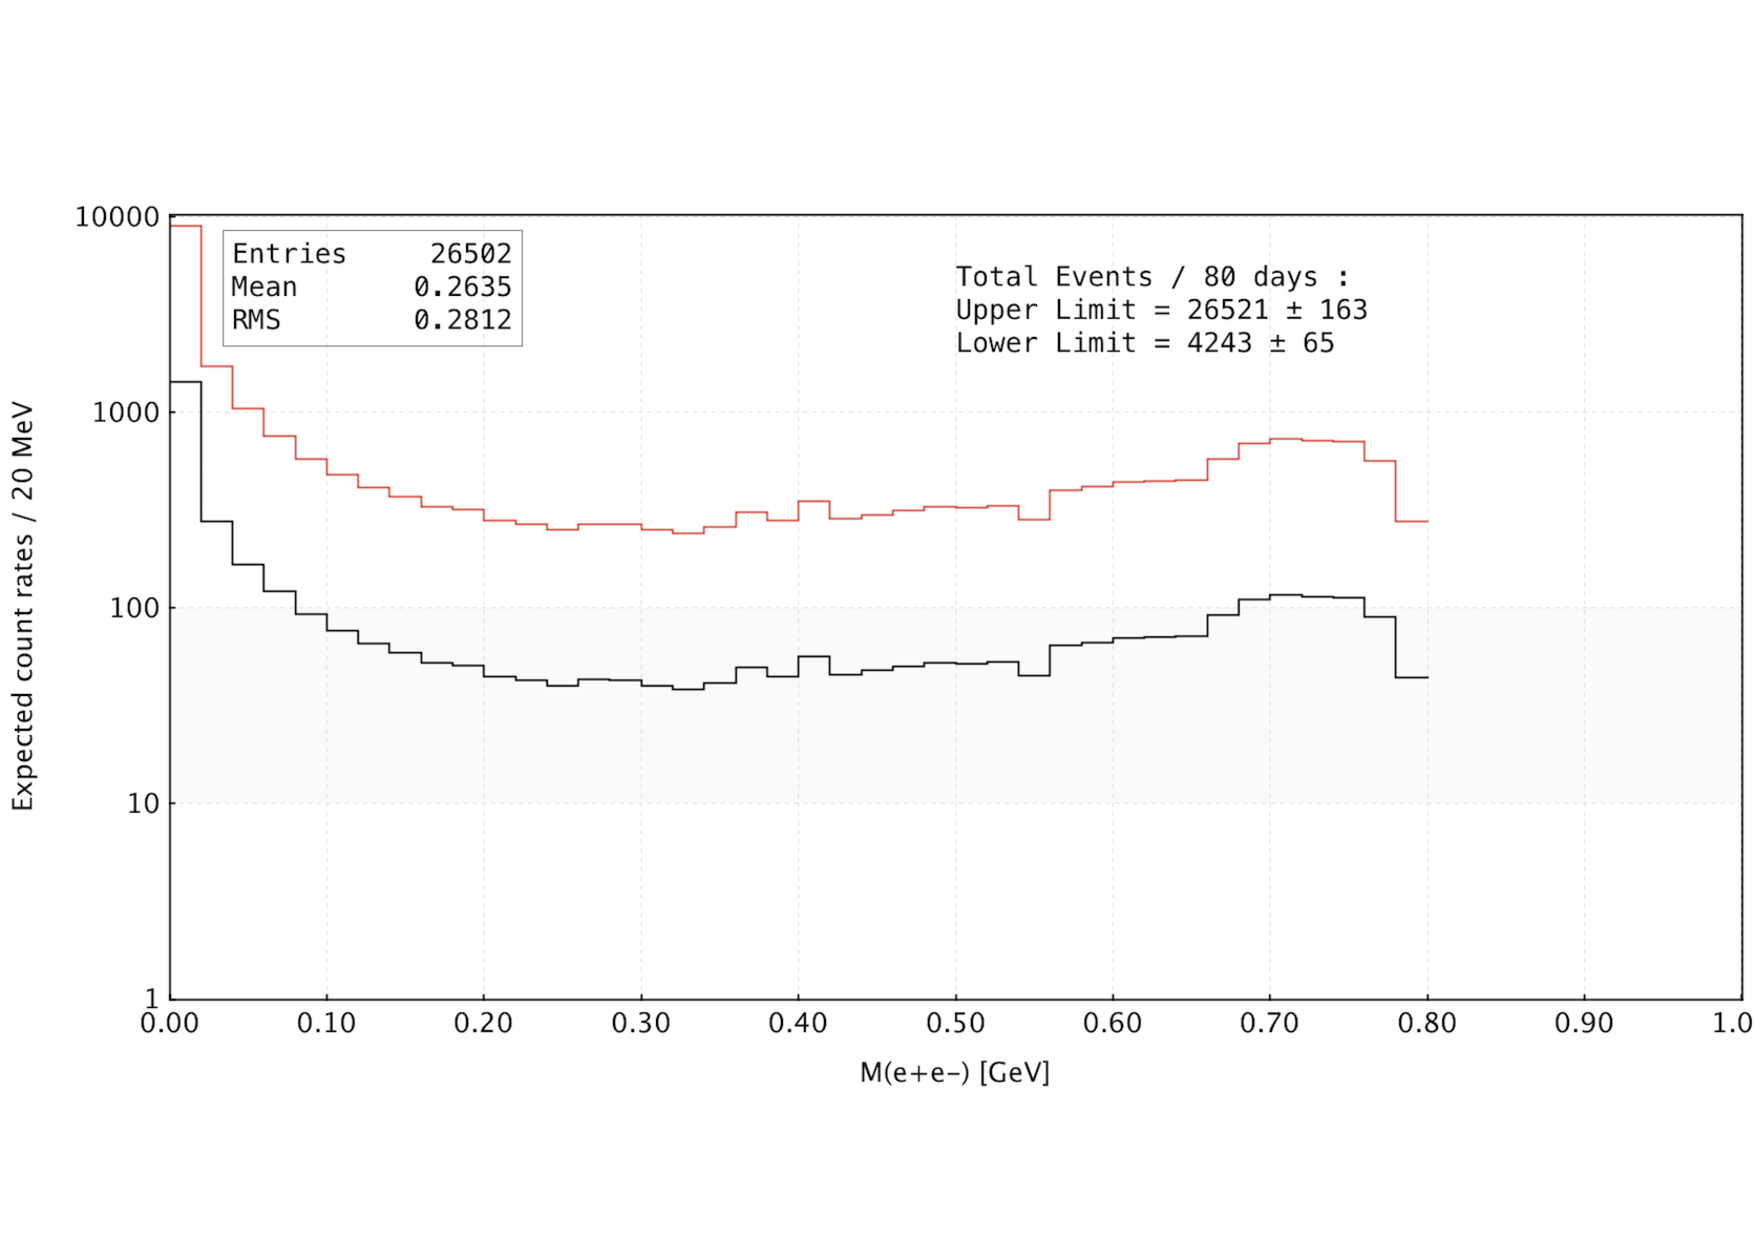
\includegraphics[width=0.8\columnwidth,height=1.0\qfigheight]{\grpath/counts/75_TORUS/VMD/VMD_Incluvise_count_rate.pdf}\label{fig:etap_count_inclu}
%	}
%\caption[Counts rates for \etaTP]{\label{fig:etayield}Count rates for the exclusive~\subref{fig:etap_count_exclu} and inclusive~\subref{fig:etap_count_inclu}. For both plots the photon detection efficiency was assumed to be between 10\%(Red) and  2\%(Black). }
%\end{center}\end{figure}
%\FloatBarrier
%Integrating over $M(\epem)$, the expected yield calculates to be $17,398$ events for exclusive scheme and $26,521$ events for the inclusive scheme. This would increase the world statistics by a factor of $\sim 20$ and $\sim 30$ respectively. 
%Table~\ref{tab:counts} and Tab.~\ref{tab:countsfull} in App.~\ref{sec:app.rates} depicts the upper and lower amount of \epemT expected from 80 days of beam time for two torus fields of 75\% and 100\% respectively.
%\FloatBarrier
%%\subsection{Realistic Yield}
%%As a reality check, lets compute the number of $\etaP \to \epem \gamma$ that g12 would have seen, had the experiment ran for 80 days with a real photon flux as calculated for CLAS12 (Sec.~\ref{sec:calflux}). %with the \epemT trigger configuration
%%The 89 $\etaP \to \epem \gamma$ events produced in g12 were recorded when the \epemT trigger was established. This time was 66\% of the total 44 days, which is $\sim29$ days. The total integrated flux measured during this time was $\sim 8.8\cdot 10^{13}$ photons. Therefore, in 80 days the total integrated flux would have been $\sim 2.4\cdot 10^{14}$ and the total number of \etaPDal \ events recorded would have been 242. The ratio of g12 total flux at 80 days per CLAS12 real photon flux is $2.73\cdot 10^{16} / 2.4\cdot 10^{14} \sim 114 $. Therefore g12 would have recorded $114\cdot 242 = 27590$ \etaPDal \ events, which is consistent with what is proposed to be measured with 80days, in the inclusive reconstruction scheme for either torus field setting. See Sec.~\ref{sec:app.rates} for total count rates.
\subsection{Acceptance at 100\% Torus field}
An addition simulation was performed using the same generated data shown above, the difference being the setting of the torus magnetic field. Below, in Fig.~\ref{fig:ratio}, the ratio of the lepton acceptance for the two different torus settings is depicted.
\begin{figure}[h!]\begin{center}
 		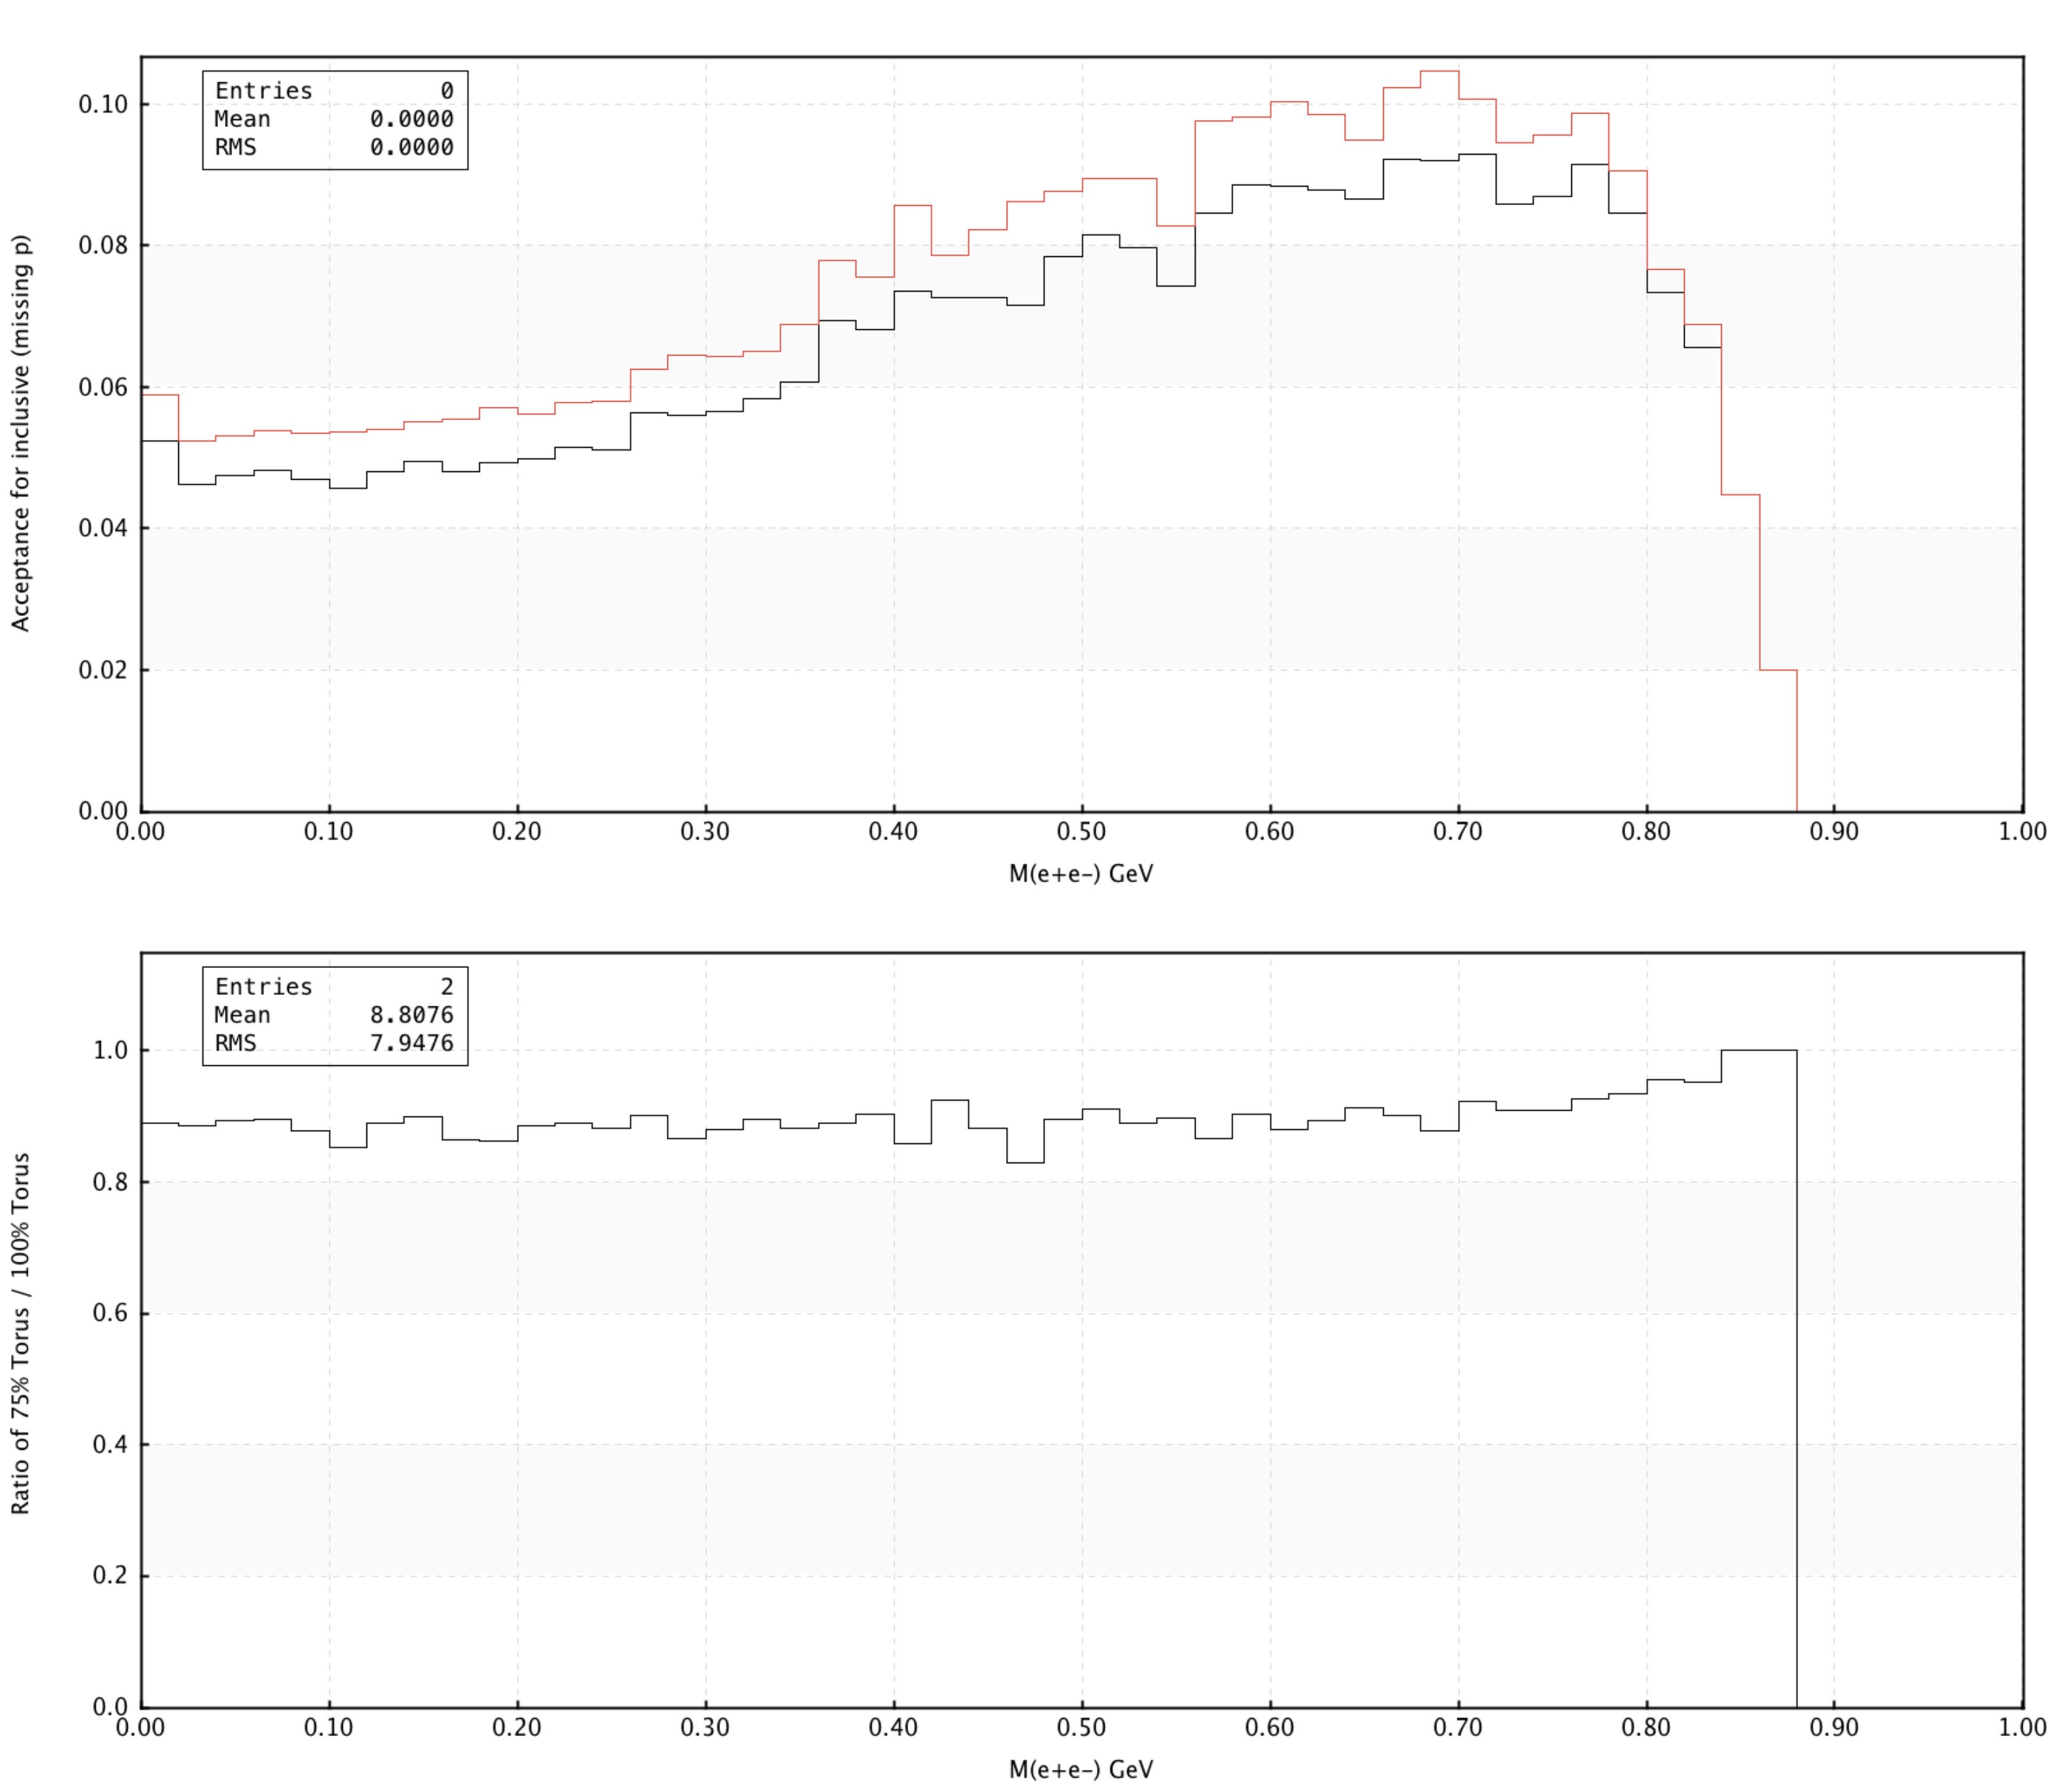
\includegraphics[width=\figwidth,height=1.6\qfigheight]{\grpath/counts/Ratio.pdf}
 		\caption[Acceptance, as a function of $M(\epem)$]{\label{fig:ratio}{Acceptance using a VMD decay model, as a function of $M(\epem)$ for the inclusive scheme(Top). The torus field was set to 75\%(red) as well as 100\%(black). Ratio of the acceptances plotted above (75\%/100\%)(Bottom). }}
\end{center}\end{figure}
\FloatBarrier
\subsection{Expected Systematic Uncertainties}
The major sources of systematic uncertainties are the acceptance and particle identification. The lepton acceptance uncertainty is estimated to be $\lesssim$ 5\% which was observed in former CLAS experiments. The lepton identification uncertainty will arise from the performance of the HTCC, PCAL and EC. From simulation studies performed for this proposal, all leptons and final state photons are detected within the geometric space of the PCAL+EC with hit coincidences in both. Furthermore, all leptons, within a few percent, that were detected in the PCAL+EC were also detected in the HTCC. Further systematics from pion contamination are mitigated by the pion rejection factor described above. Systematics related to external photon conversion are minimal due to the  1~mm resolution of the primary vertex given by the Silicon Vertex Tracker (SVT) as shown in Sec~\ref{sec:intro.conversion}. Any Bethe-Heitler contributions are negligible when utilizing and exclusive meson reconstruction scheme.




%\section{Summary}
\section{Appendix}\label{sec:app}

\subsection{$\etaP$ Decays}\label{sec:decays}
 Figure~\ref{fig:piz.alldecay} illustrates the Feynman diagrams for the ``Two photon decay'' and the ``Dalitz decay''.
%Table~\ref{tab:pi0}. Figure~\ref{fig:piz.alldecay} illustrates the Feynman diagrams for the ``Two photon decay'' and the ``Dalitz decay''.
\begin{figure}[h!]\begin{center}
\subfloat[Feynman Diagram of $\etaP$ Two Photon Decay][]{ %Feynman diagram of $\etaP$ two photon decay
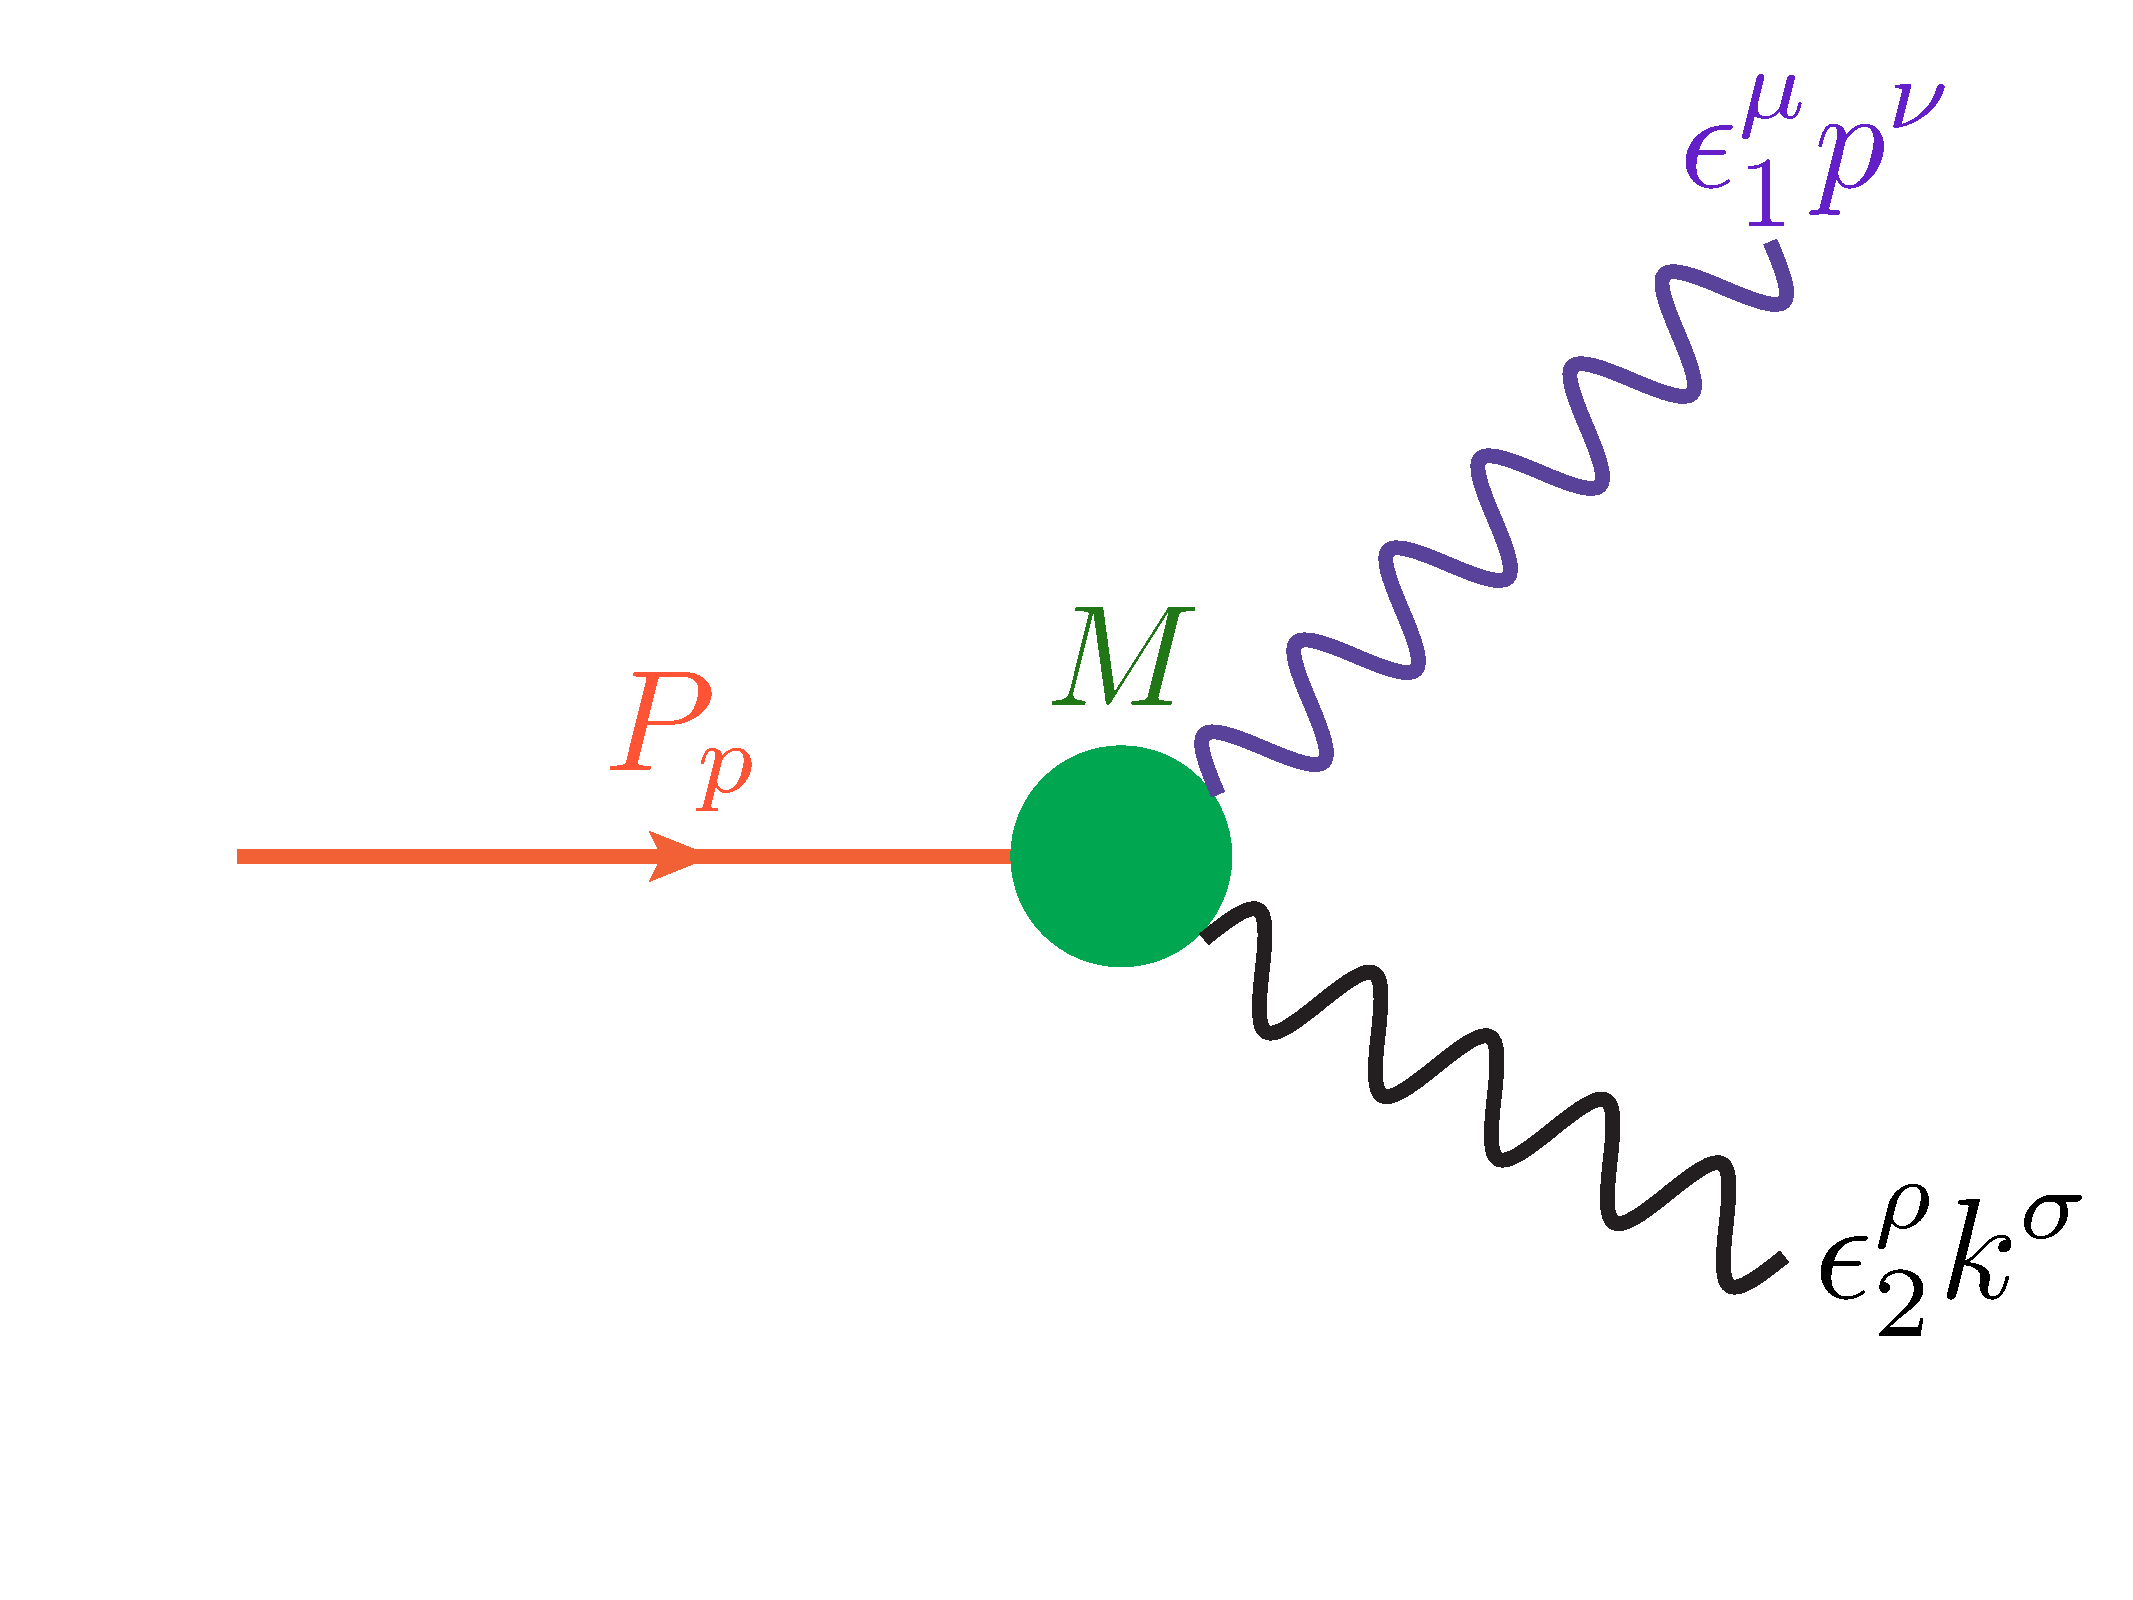
\includegraphics[width=0.65\columnwidth,height=0.65\qfigheight]{\grpath/decays/P_to_gamgam_wnotation.pdf}\label{fig:piz.gamgam}
}

\subfloat[Feynman Diagram of $\etaP$ Dalitz Decay][]{ %Feynman diagram of $\etaP$ Dalitz decay
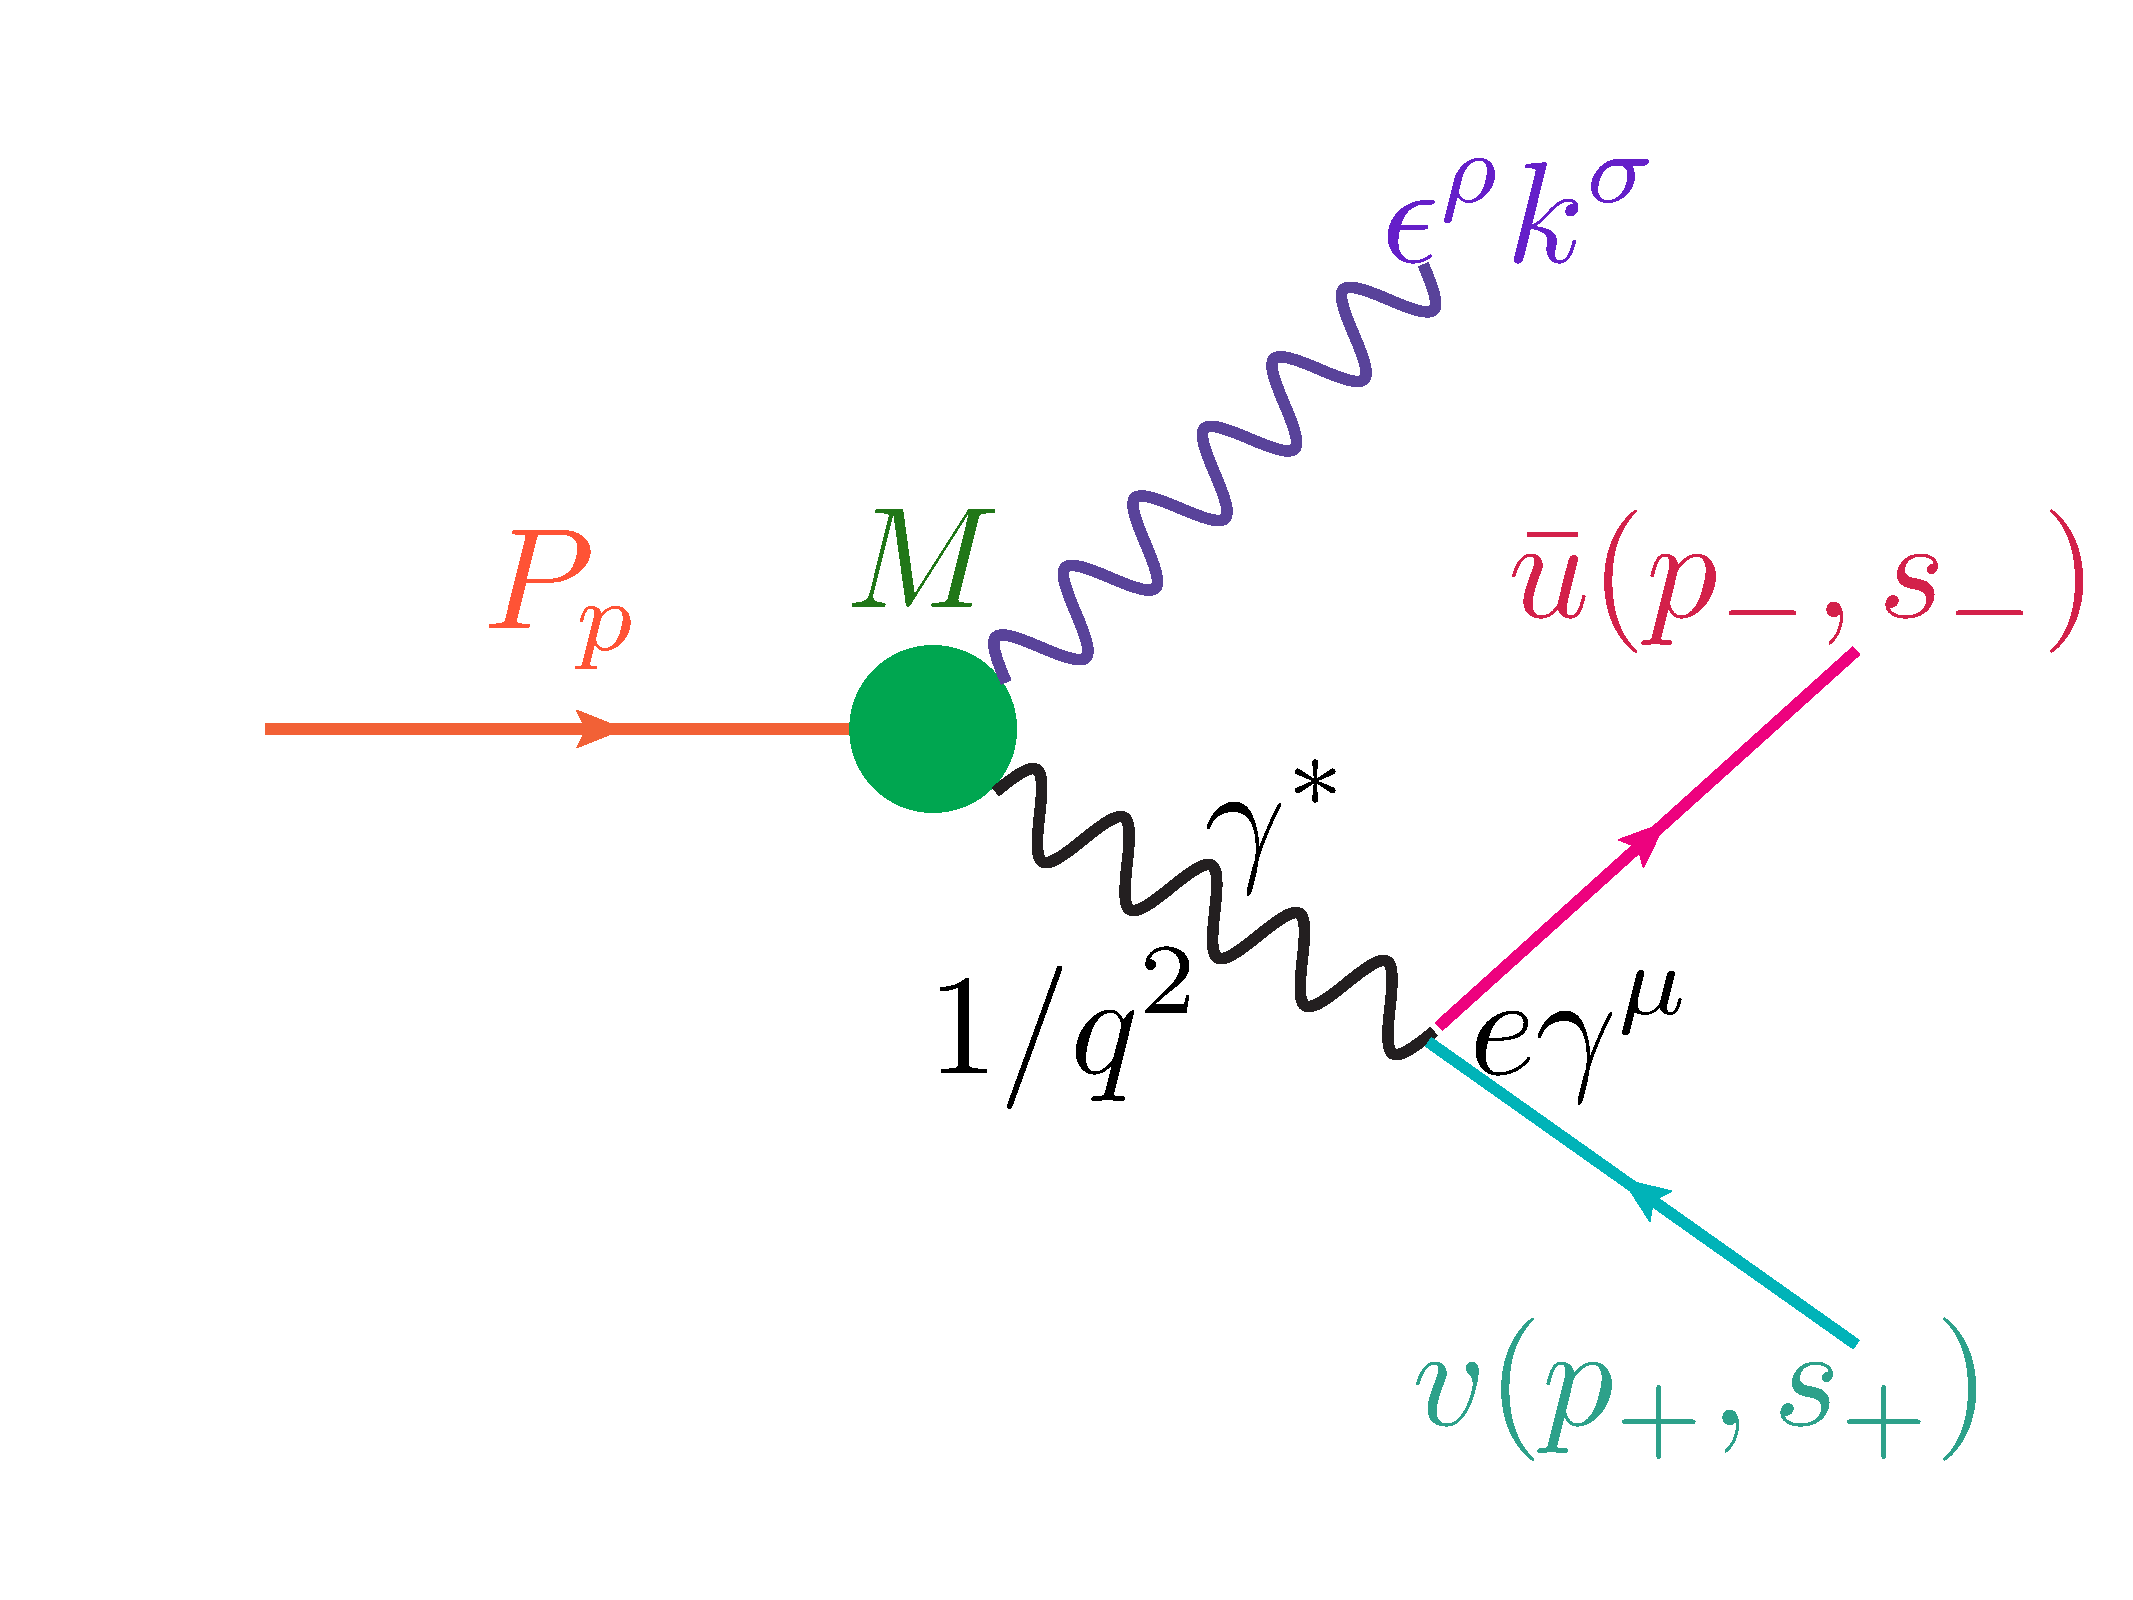
\includegraphics[width=0.65\columnwidth,height=0.65\qfigheight]{\grpath/decays/P_to_lepsgam_wnotation.pdf}\label{fig:piz.dalitz}
}
\caption[Feynman diagram of $P_p$($\etaP$) two photon decay and Dalitz decay]{\label{fig:piz.alldecay}Feynman diagram of $P_p$($\etaP$) two photon decay~\subref{fig:piz.gamgam}, $\epsilon_1$ and $\epsilon_2$ are the polarizations, $p$ and $k$ are 4-momenta of the photons.  Feynman diagram of $P_p$($\pi^0$) Dalitz decay~\subref{fig:piz.dalitz}, the variable $s_\pm$ are the spin helicities of the outgoing leptons $l^\pm$ with 4-momenta $p_{\pm}$ and $\epsilon$ is the polarization of the outgoing photon with 4-momenta $k$. In both diagrams $\mathcal{M}$ is the form factor.}

\end{center}\end{figure}
%\FloatBarrier
\subsection{Two Photon Decay}\label{sec:piz.gg}
As shown in Fig.~\ref{fig:piz.gamgam}, the two photon decay can be expressed in terms of the respective momentum, $P_p$($\eta^{\prime}$)$\to \gamma(\epsilon_1,p) \gamma(\epsilon_2,k)$, where $\epsilon_1$ and $\epsilon_2$ are the polarizations of the photons with 4-momenta $p$ and $k$. Dropping the nomenclature ($\eta^{\prime}$) in $P_p$($\eta^{\prime}$), the four momentum of the decaying meson is $P_p= p+k$. Using the Feynman rules as given in~\cite{peskin}and~\cite{halzen}, which are Lorentz and gauge invariant and also parity conserving, the amplitude can be solved to be:

\begin{align}\label{eq:piz.gg.amp}
 {\cal M}(P_P \to \gamma(\epsilon_1,p) \gamma(\epsilon_2,k))= {M}_P(p^2=0,k^2=0) \varepsilon_{\mu\nu\rho\sigma}\epsilon_1^\mu p^\nu \epsilon_2^\rho k^\sigma
\end{align}
where $\varepsilon_{\mu\nu\rho\sigma}$ is the antisymmetric metric tensor. The form factor, ${M}_P(p^2=0,k^2=0)$, contains information of the decaying meson and since the decay products are on-shell photons, which are massless, ${M}_P$ is a constant given as;
\begin{align}\label{eq:decay.constants}
 {M}_P=\begin{cases}
         {\displaystyle\frac{\alpha}{\pi f_{\pi}}} & \mbox{if $P=\etaP$};\\
        {\displaystyle\frac{\alpha}{\pi f_\pi} \frac{1}{\sqrt{3}} }\left( \frac{f_\pi}{f_8} \cos\theta_{mix} -2\sqrt{2} \frac{f_\pi}{f_0} \sin\theta_{mix} \right)& \mbox{if $P=\eta$};\\
        {\displaystyle\frac{\alpha}{\pi f_\pi} \frac{1}{\sqrt{3}}} \left( \frac{f_\pi}{f_8} \sin\theta_{mix} +2\sqrt{2} \frac{f_\pi}{f_0} \cos\theta_{mix} \right)& \mbox{if $P=\eta'$} \,
\end{cases}
\end{align}
where $\alpha=e^2/4\pi \approx 1/137$ is the fine structure constant, $f_\pi \approx 92.4 \,{\rm MeV}$ is the physical value of the pion-decay constant and $f_0 \approx 1.04 f_\pi$ and $f_8 \approx 1.3 f_\pi$ are the singlet and octet Pseudo-Goldstone meson decay constants.

\subsubsection{\emph{Squared Matrix Element}}
The squared matrix element of the decay $P_P \to \gamma(\epsilon_1,p) \gamma(\epsilon_2,k)$ is given by
\begin{align}\label{eq:piz.gg}
\left|{\cal  M}(P_{P}\rightarrow\gamma(\epsilon_{1},p)\gamma(\epsilon_{2},k))\right|^{2}=\left|M_{P}\right|^{2}\varepsilon_{\mu\nu\rho\sigma}\varepsilon_{\mu^{\prime}\nu^{\prime}\rho^{\prime}\sigma^{\prime}}\epsilon_{1}^{\mu}p^{\nu}\epsilon_{2}^{\rho}k^{\sigma}\epsilon_{1}^{\mu^{\prime}}p^{\nu^{\prime}}\epsilon_{2}^{\rho^{\prime}}k^{\sigma^{\prime}}
%
\end{align}
which can be simplified to;
\begin{align}\label{eq:piz.gg.simplify}
\left|{\cal M}(P_{P}\to\gamma(p)\gamma(k))\right|^{2}=\left|M_{P}\right|^{2}\varepsilon_{\mu\nu\rho\sigma}\varepsilon^{\mu\nu}_{\quad \rho^{\prime}\sigma^{\prime}}p^{\rho}p^{\rho^{\prime}}k^{\sigma}k^{\sigma^{\prime}}
%
\end{align}
by assuming that the polarizations of the photons remain unobserved, as they are in \abbr{CLAS}. Therefore the photon polarization vectors can be summed using Eq.~5.75 from~\cite{peskin} which reads as;
\begin{align}
\sum\limits_{polarizations} \epsilon_{\mu} \epsilon_{\mu^{\prime}} \to -g_{\mu\mu^{\prime}} 
\end{align}
As indicated in ~\cite{peskin}, the right arrow indicates that this is not an actual equality, but the solution is valid as long as both sides are dotted into Eq.~\ref{eq:piz.gg}. The antisymmetric tensor, $\varepsilon_{\mu\nu\rho\sigma}\varepsilon^{\mu\nu}_{\quad \rho^{\prime}\sigma^{\prime}}$ is simplified using  Eq.~A.30 of \cite{peskin}; 
\begin{align}\label{eg:antiT_ID}
\varepsilon_{\mu\nu\rho\sigma}\varepsilon^{\mu\nu}_{\quad \rho^{\prime}\sigma^{\prime}} = -2(g_{\rho\rho^{\prime}}g_{\sigma\sigma^{\prime}} - g_{\rho\sigma^{\prime}}g_{\rho^{\prime}\sigma})\\
\end{align}
Applying Eq.~\ref{eg:antiT_ID} to Eq.~\ref{eq:piz.gg.simplify} results in;
\begin{align}\label{eq:piz.gg.reduced}
\left|{\cal M}(P_{P}\to\gamma(p)\gamma(k))\right|^{2}=\left|M_{P}\right|^{2}(-2)(p^2k^2 - (p\cdot k)^2) \ .
%
\end{align}
Substituting
\begin{align}
(p + k)^2 = p^2 + k^2 +2 (p\cdot k) \ ,
\end{align}
and applying $p^2= k^2=0$, since both photons are massless because they are on-shell, we can derive the final expression of the squared amplitude of the decay $P_P \to \gamma(\epsilon_1,p) \gamma(\epsilon_2,k)$ as;
\begin{align}\label{eq:piz_gg_amp_final}
\left|{\cal M}(P_{P}\to\gamma(p)\gamma(k))\right|^{2}= \left|M_{P}\right|^{2}\frac{1}{2}(p+k)^{4} = \frac{1}{2}\left|M_{P}\right|^{2}m_{P}^{4}
\end{align}
where $m_P^4$ is the mass of the \etaTP derived from the 4-momenta conservation equation $(p+k)^4 = m_P^4$
\subsubsection{\emph{Decay rate}}
The decay rate of a two-body decay is explained in Equation 46.17 of~\cite{pdg2014} as
\begin{align}\label{eq:pdg.2body}
d\Gamma = \frac{1}{32 \pi^2} A \left|{\cal M}\right|^2\frac{\left|\bf{p_1}\right|}{m_p^2}d\Omega \ ,
\end{align}
where $d\Omega$ is the solid angle of particle 1 and $A$ is the symmetry factor which appears because of the Bose symmetry of the two
outgoing photons. Substituting the square matrix element from Eq.~\ref{eq:piz_gg_amp_final} into Eq.~\ref{eq:pdg.2body} and integrating over the solid angle yields;
\begin{align}
\Gamma_{P\rightarrow\gamma\gamma} = \frac{1}{32\pi^{2}} \frac{1}{2} \left|{\cal M}(P_{P}\to\gamma(p)\gamma(k))\right|^{2} \frac{\left|\bf{p}\right|}{m_{P}^2} 4 \pi = \frac{1}{32 \pi}\left|M_{P}\right|^{2}m_{P}^{2}\left|\bf{p}\right|
\end{align} 
Finally, in the center-of-mass (C.M.) frame of the decaying meson, $\bf{p} = E_{\gamma}^{C.M.} = \frac{m_p}{2}$, we find the final expression of the decay rate of $P_P \to \gamma(\epsilon_1,p) \gamma(\epsilon_2,k)$ as;
\begin{align}\label{eq:piz.gg.decay.final}
\Gamma_{P\rightarrow\gamma\gamma} = \frac{1}{64\pi} \left|M_{P}\right|^{2}m_{P}^{3} \ .
\end{align}


%
\subsubsection{\emph{Photon Conversion to \epem Pairs}}\label{sec:intro.conversion}
When a photon travels through matter at energies greater than 100~MeV, it can convert into an electron-positron pair. The process of pair production, $\gamma Z \rightarrow Ze^{+}e^{-}$, occurs when a photon with $E_0 > 2 m_e c^2$ converts into an electron and a positron. The cross section for this process can be written as;
\begin{equation}\label{pair_crosssection}
\sigma_{\gamma\rightarrow e^+e^-} =  \frac{A}{N_{A} \rho \lambda_\gamma}  \ ,\ \lambda_\gamma = \frac{9}{7}X_0
\end{equation}
where $\lambda$ is the interaction length, or mean free path, $\rho$ is the density of the material, $N_A$ is Avogadro's number and $A$ is the atomic mass of the material. The probability of pair production to occur is solely based on $X_{0}$, the radiation length of the medium and this probability can be expressed as;
\begin{equation}
\frac{dP}{dx} = \frac{1}{\lambda_\gamma}\exp(\frac{-x}{\lambda_\gamma}) \ .
\end{equation}
%
%
The probability of pair production when a photon, from the $\etaP \to \gamma \gamma$ decay, traveling though 5~cm of liquid hydrogen, $\ell$H$_2$, is shown in Fig.~\ref{fig:conversion}. 
\begin{figure}[h!]\begin{center}
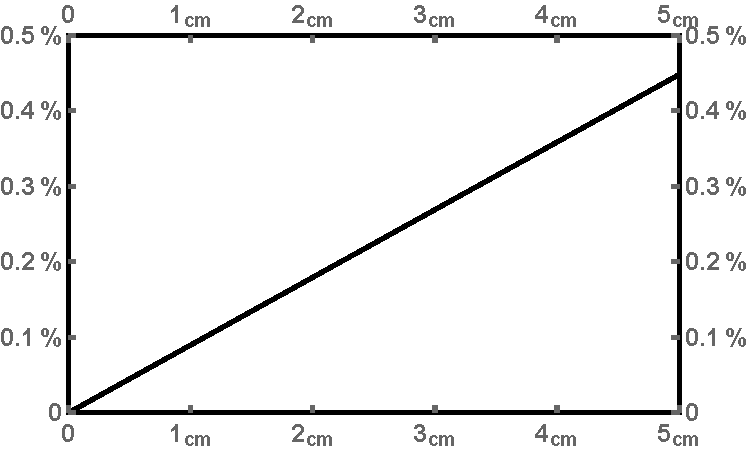
\includegraphics[width=\figwidth,height=\qfigheight]{\grpath/decays/Hydrogen_conversion_Prob_CLAS12.pdf}
\caption[Probability of pair production, $\gamma \to$\epem, as a function of distance in liquid hydrogen]{\label{fig:conversion}{Probability of pair production, $\gamma \to$\epem, as a function of distance in liquid hydrogen.}}
\end{center}\end{figure}
Since CLAS12 has a vertex resolution of $\approx$1~mm the probability of pair production traveling through 10~mm is shown in Fig.~\ref{fig:conversionmm}. 
\begin{figure}[h!]\begin{center}
		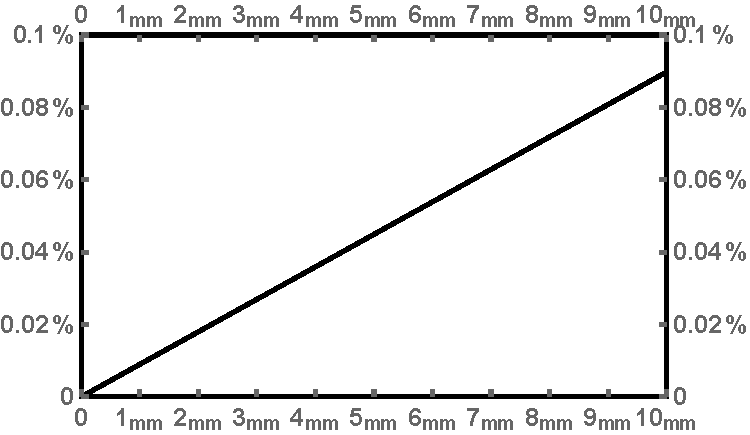
\includegraphics[width=\figwidth,height=\qfigheight]{\grpath/decays/Hydrogen_conversion_Prob_CLAS12mm.pdf}
		\caption[Probability of pair production, $\gamma \to$\epem, as a function of distance in liquid hydrogen]{\label{fig:conversionmm}{Probability of pair production, $\gamma \to$\epem, as a function of distance in liquid hydrogen.}}
	\end{center}\end{figure}
This type of subprocess mimics the Dalitz decay  $\etaP \to e^+e^- \gamma$, described in Sec.~\ref{sec:dalitzdecay}. Since there are 2 photons with equal probability of conversion, the total probability is double that shown in Fig.~\ref{fig:conversion}.



%\subsection{$\etaP$ Dalitz Decay}\label{sec:dalitzdecay} 
When a pseudoscalar meson decays via a photon $\gamma$ and a dilepton ($l^{+}l^{-}$) pair, it is known as a Dalitz decay or a so-called single off-shell decay. The Dalitz decay is related to the two photon decay. However, in the Dalitz decay, one of the photons is off-shell ($\gamma^*$) and decays into a dilepton pair. Since the Dalitz decay is related to the two photon decay, the form factor of the Dalitz decay, for P($\eta'$), will be similar to the form factor of the two photon decay of P( $\eta'$), except there will be an effective mass dependence for the Dalitz decay. Figure~\ref{fig:piz.dalitz} depicts the Feymann diagram of the Dalitz decay.

The amplitude for the decay $P_P \to \gamma^\star(p) \gamma(k) \to l^+(p_+)l^-(p_-) \gamma(k)$ is given by the following expression:
\begin{align}\label{eq:piz.eeg.amp}
{\cal M}(P\to l^+(p_+,s_+)l^-(p_-,s_-) \gamma) = &{M}_P(p^2,k^2=0) \varepsilon_{\mu\nu\rho\sigma} \frac{1}{q^2} \nonumber \times \left[\right. \\ 
&\left. e \bar u(p_-,s_-) \gamma^\mu v(p_+,s_-) q^\nu \epsilon^\rho k^\sigma \right] .
\end{align}
Comparing the amplitudes of Eq.~\ref{eq:piz.eeg.amp} and Eq.~\ref{eq:piz.gg.amp} it is seen that the polarization of the off-shell photon turned into the current $e \bar u(p_-,s_-) \gamma^\mu v(p_+,s_-)$ of the lepton pair. The parameters $s_\pm$ are the spin helicities of the outgoing leptons $l^\pm$ and as in  Eq.~\ref{eq:piz.gg}, $\epsilon$ is the polarization of the outgoing photon. 
%
\subsubsection{\emph{Squared Matrix Element}}


\begin{align}\label{eq:piz.eeg}
&\left|{\cal M}(P\to l^+(p_+,s_+)l^-(p_-,s_-) \gamma)\right|^2 =  \frac{e^2}{q^4} \left|M\right|^2  \varepsilon_{\mu\nu\rho\sigma}\varepsilon_{\mu^{\prime}\nu^{\prime}\rho^{\prime}\sigma^{\prime}}   \nonumber \times \left[\right.
\\ & \left.\bar u(p_-,s_-) \gamma^\mu v(p_+,s_+) \bar v(p_+,s_+) \gamma^{\mu^{\prime}}  u(p_-,s_-) q^\nu \epsilon^\rho k^\sigma q^{\nu^{\prime}} \epsilon^{\rho^{\prime}} k^{\sigma^{\prime}}\right] .
%
\end{align}
using an equation found between equation 5.3 and 5.4 found in~\cite{peskin}
\begin{align}\label{eq:spin.sum}
& \sum\limits_{s_{-},s_{+}}^{} \bar{u}(p_{-},s_{-})\gamma^{\mu}\nu(p_{+},s_{+})\bar{\nu}(p_{+},s_{+})\gamma^{\mu^{\prime}}u(p_{-},s_{-}) = Tr\left[ (\slashed{p}_- +m)\gamma^{\mu} (\slashed{p}_+-m)\gamma^{\mu^{\prime}} \right]\nonumber \\ & =2q^{2}\left[-(g_{\mu\mu^{\prime}}-\frac{p_{\mu}p_{\mu^{\prime}}}{q^{2}} ) - \frac{(p_{+} - p_{-})_{\mu}(p_{+} - p_{-})_{\mu^{\prime}}}{q^{2}}\right]
\end{align}
where the identity $q = p_+ + p_-$ was used.
Substituting Eq.~\ref{eq:spin.sum} into Eq.~\ref{eq:piz.eeg}
\begin{align} \label{eq:piz.eeg.midway1}
\left|{\cal M}\right|^{2} = &  \frac{2e^{2}\left|M_{P}\right|^{2}}{q^{2}}\varepsilon_{\mu\nu\rho\sigma}\varepsilon_{\mu^{\prime}\nu^{\prime}\rho^{\prime}\sigma^{\prime}}\left[-g^{\mu\mu^{\prime}} - \frac{(p_{+} - p_{-})^{\mu}(p_{+} - p_{-})^{\mu^{\prime}}}{q^{2}}\right]
\times \nonumber \\ &\left[ (-g^{\nu\nu^{\prime}})q^{\rho}k^{\sigma}q^{\rho^{\prime}}k^{\sigma^{\prime}} \right]
\end{align}
Substituting $k = P - q$ and $p_- = q - p_+$ into Eq.~\ref{eq:piz.eeg.midway1}
\begin{align} \label{eq:piz.eeg.midway2}
\left|{\cal M}\right|^{2} = & \frac{2e^{2}\left|M_{P}\right|^{2}}{q^{2}}\varepsilon_{\mu\nu\rho\sigma}\varepsilon_{\mu^{\prime}\nu^{\prime}\rho^{\prime}\sigma^{\prime}}\left[-g^{\mu\mu^{\prime}} - \frac{(2p_{+} - q)^{\mu}(2p_{+} - q)^{\mu^{\prime}}}{q^{2}}\right] \times \nonumber \\ &  (-g^{\nu\nu^{\prime}})      
(q^{\rho}P^{\sigma} - q^{\rho}q^{\sigma}) (q^{\rho}P^{\sigma^{\prime}} - q^{\rho^{\prime}}q^{\sigma^{\prime}})
\end{align}
Applying properties of $-g^{\mu\mu^{\prime}}$ and $-g^{\nu\nu^{\prime}}$ onto Eq.~\ref{eq:piz.eeg.midway2}
\begin{align} \label{eq:piz.eeg.midway3}
\left|{\cal M}\right|^{2} = \frac{2e^{2}\left|M_{P}\right|^{2}}{q^{2}}
& \left[\varepsilon_{\mu\nu\rho\sigma}\varepsilon^{\mu\nu}_{\quad \rho^{\prime}\sigma^{\prime}}q^{\rho}P^{\sigma}q^{\rho^{\prime}}P^{\sigma^{\prime}} +
\right. \nonumber \\ & \left. \frac{4}{q^2} \varepsilon_{\mu\nu\rho\sigma}\varepsilon^{\mu}_{\ \ \nu^{\prime} \rho^{\prime}\sigma^{\prime}} p_{+}^{\nu}p_{+}^{\nu^{\prime}}q^{\rho}q^{\rho^{\prime}}P^{\sigma}P^{\sigma^{\prime}}\right]
\end{align}
Switching to the rest frame of the pseudoscalar meson, $P_p$, the 4-momenta is transformed to $P^\sigma = m_p\delta^{\sigma 0}$. The squared amplitude of Eq.~\ref{eq:piz.eeg.midway3} reads;
\begin{align} \label{eq:piz.eeg.midway4}
\left|{\cal M}\right|^{2} = & \frac{2e^{2}\left|M_{P}\right|^{2}}{q^{2}}m_p^2
\left[\varepsilon_{\mu\nu\rho}\varepsilon^{\mu\nu}_{\ \ \rho^{\prime}}q^{\rho}q^{\rho^{\prime}} - \frac{4}{q^2} \varepsilon_{\mu\nu\rho}\varepsilon^{\mu}_{\ \nu^{\prime}\rho^{\prime}} p_{+}^{\nu}p_{+}^{\nu^{\prime}}q^{\rho}q^{\rho^{\prime}}\right]
\end{align}
The sign change is due to $g^{\sigma \sigma^{\prime}} = -\delta^{\sigma \sigma^{\prime}}$. 
Using the antisymmetric tensor properties $\varepsilon_{\mu\nu\rho}\varepsilon^{\mu\nu}_{\ \ \rho^{\prime}} = 2\delta_{\rho\rho^{\prime}}$ and $\varepsilon_{\mu\nu\rho}\varepsilon^{\mu}_{\ \nu^{\prime}\rho^{\prime}} = \delta_{\nu\nu^{\prime}}\delta_{\rho\rho^{\prime}} - \delta_{\nu\rho^{\prime}}\delta_{\rho\nu^{\prime}} = (\hat{e}_{\nu} \times \hat{e}_{\rho}) \cdot (\hat{e}_{\nu^{\prime}} \times \hat{e}_{\rho^{\prime}})$, Eq.~\ref{eq:piz.eeg.midway4} is reduced to 
\begin{align} \label{eq:piz.eeg.final}
\left|{\cal M}\right|^{2} =  \frac{2e^{2}\left|M_{P}\right|^{2}}{q^{2}}m_p^2
\left[2\left|\bf{q}\right|^2 - \frac{4}{q^2} \left|\bf{q}\right|^2 \left|\bf{p_{+}}\right|^2 \sin^2(\theta_{p_{_+}q}) \right]
\end{align}

\subsubsection{\emph{Decay rate}}
The decay rate of a three-body decay is given in Equation 46.19 of~\cite{pdg2014} as
\begin{align}\label{eq:pdg.3body}
d\Gamma = \frac{1}{(2 \pi)^5} \frac{1}{16 m_p^2} \left|{\cal M}\right|^2 \left|\bf{p_1^*}\right| \left|\bf{p_3}\right|d\Omega_1^*d\Omega_3 dm_{12} \ ,
\end{align}
%
where ($\left|\bf{p_1^*}\right|,\Omega_1^*$) is the momentum of particle 1 in the rest frame of 1 and 2, and $\Omega_3$ is the angle of particle 3 in the rest frame of the decaying particle $m_p$~\cite{pdg2014}. Relating Eq.~\ref{eq:pdg.3body} to the variables in Eq.~\ref{eq:piz.eeg.final}, where $(\left|\bf{p_1^*}\right|,\Omega_1^*) = (\left|\bf{p_+}\right|,\Omega_{p_{_+}q})$, $m_{12} = q$ and $(\left|\bf{p_3}\right|,\Omega_3) = (\left|\bf{p_k}\right|,\Omega_k)$, reads;
\begin{align}\label{eq:pdg.3body.sub}
d\Gamma = \frac{1}{(2 \pi)^5} \frac{1}{16 m_p^2} \left|{\cal M}\right|^2 \left|\bf{p_+}\right| \left|\bf{p_k}\right|d\Omega_+d\Omega_k dq \ ,
\end{align}
%
In the rest from of the decaying particle $m_p$, the 3-momenta $\left|\bf{p_k}\right| = \left|\bf{q}\right|$ and the solid angle $\Omega_k = \Omega_q$. Substituting the square matrix element from Eq.~\ref{eq:piz.eeg.final} into Eq.~\ref{eq:pdg.3body.sub} yields;
%
\begin{align}\label{eq:pdg.3body.sub2}
d\Gamma = & \frac{1}{(2 \pi)^5} \frac{1}{16 m_p^2} \frac{2e^{2}\left|M_{P}\right|^{2}}{q^{2}}m_p^2
\left[2\left|\bf{q}\right|^2 - \frac{4}{q^2} \left|\bf{q}\right|^2 \left|\bf{p_{+}}\right|^2 \sin^2(\theta_{p_{_+}q}) \right]
 \times \left[ \nonumber \right. \\ &\left. \left|\bf{p_+}\right| \left|\bf{q}\right|d\Omega_{p_{_+}q}d\Omega_q dq\ \right].
\end{align}
The variables $\left|\bf{q}\right|$ and $\left|\bf{p_+}\right|$ can be redefined, by means of Eq.~46.20b and Eq.~46.20a of~\cite{pdg2014}, as 
\begin{align}
\left|\bf{q}\right| = \frac{m_p^2 - q^2}{2m_p} \label{eq:eeg.qeq} \\
\left|\bf{p_+}\right| = \frac{\sqrt{q^2 - 4m_l^2}}{2} = \frac{q\sqrt{1 - \frac{4m_l^2}{q^2} } } {2} =\frac{q {\cal K}  } {2}  \label{eq:eeg.p+eq} \ ,
\end{align} 
where ${\cal K} = \sqrt{1 - \frac{4m_l^2}{q^2}}$. Replacing the variables calculated in Eq.~\ref{eq:eeg.qeq} and Eq.~\ref{eq:eeg.p+eq} into Eq.~\ref{eq:pdg.3body.sub2} and collecting terms yields;
\begin{align}\label{eq:pdg.3body.sub3}
d\Gamma = \frac{1}{(2 \pi)^5} \frac{1}{16 m_p^2} \left|M_{P}\right|^{2} & \left[ \frac{2e^2 m_p^2}{8} \left( \frac{m_p^2 - q^2}{2 m_p}\right)^3\right] \times \nonumber \left[ \right. \\ &  \left.
\left( 2 -{\cal K}^2\sin^2(\theta_{p_{_+}q})\right)\frac{{\cal K}}{4 q^2}dq^2d\Omega_{p_{_+}q}d\Omega_q \right] \ ,
\end{align}
where the identity $qdq = \frac{dq^2}{2}$. Performing the integration of $\Omega_{p_{_+}q}d\Omega_q$ and replacing $e^2 = 4\pi\alpha$ transforms Eq.~\ref{eq:pdg.3body.sub3} into;
\begin{align}\label{eq:pdg.3body.sub4}
d\Gamma = \frac{1}{(2 \pi)^3} \frac{1}{32} \frac{4 \pi \alpha}{3} \left|M_{P}\right|^{2} \left[ \frac{m_p^6 \left( 1- \frac{q^2}{m_p^2}\right)^3}{m_p^3} \right]\left( 3 -{\cal K}^2\right)\frac{{\cal K}}{q^2}dq^2\ ,
\end{align}
which can be simplified further to;
\begin{align}\label{eq:eeg.final}
d\Gamma = \left(\frac{1}{64\pi} \left|M_{P}\right|^{2}m_{P}^{3} \right) \frac{2 \alpha}{3 \pi} \frac{1}{q^2} \left( 1- \frac{q^2}{m_p^2}\right)^3 \left( 1+ \frac{2m_l^2}{q^2}\right) \left( 1- \frac{4m_l^2}{q^2}\right)^{\frac{1}{2}} dq^2\ .
\end{align}
It can be seen that the first set of variables in parenthesis in Eq.~\ref{eq:eeg.final} is Eq.~\ref{eq:piz.gg.decay.final}, therefore;
\begin{align}\label{eq:eegff.finalkroll}
\frac{d\Gamma}{\Gamma_{\gamma\gamma} dq^2} = \frac{2 \alpha}{3 \pi} \frac{1}{q^2} \left( 1- \frac{q^2}{m_p^2}\right)^3 \left( 1+ \frac{2m_l^2}{q^2}\right) \left( 1- \frac{4m_l^2}{q^2}\right)^{\frac{1}{2}} 
\end{align}
which is the Kroll-Wada equation founded in~\cite{KrollWada}.
%\subsection{$\phi$ Dalitz Decay}\label{sec:phidalitzdecay} 
%%When the $\phi$ meson decays via a $\eta$ and a dilepton ($l^{+}l^{-}$) pair, it is also known as a Dalitz decay or a so-called single off-shell decay. This Dalitz decay is related to the $\eta \gamma$ decay. However, in the Dalitz decay, one of the photons is off-shell ($\gamma^*$) and decays into a dilepton pair. Since the Dalitz decay is related to the two photon decay, the form factor of the Dalitz decay, for V($\phi$), will be similar to the form factor of the $\eta \gamma$ decay of P($\phi$), except there will be an effective mass dependence for the Dalitz decay. 
%The amplitude for the decay $V_P \to \gamma^\star(p_1) \eta(p_2) \to l^+(p_+)l^-(p_-) \eta(p_2)$ is similar Eq.~\ref{eq:piz.eeg.amp}, but replacing the on-shell photon with an $\eta$:
%\begin{equation}\label{eq:phi.eeg.amp}
%{\cal M}(P\to l^+(p_+,s_+)l^-(p_-,s_-) \eta(p_2)) = {M}_P(p_{1}^2,p_{2}^2) \varepsilon_{\mu\nu\rho\sigma} \frac{1}{q^2} e \bar u(p_-,s_-) \gamma^\mu v(p_+,s_-) q^\nu \epsilon^\rho p_{2}^\sigma.
%\end{equation}
%\subsubsection{\emph{Decay rate}}
%The decay rate for the $\phi$ transition to $\eta \gamma^\star$ is derived as~\cite{landsberg}:
%\begin{align}
%\frac{d\Gamma}{\Gamma_{\eta\gamma} dq^2} = \frac{\alpha}{3 \pi} \frac{1}{q^2} \left( \left(1+ \frac{q^2}{m_{\phi}^2 - m_{\eta}^2} \right)^2 - \frac{4 m_{\phi}^2 q^2}{m_{\phi}^2 - m_{\eta}^2}\right)^\frac{3}{2} \left( 1+ \frac{2m_l^2}{q^2}\right) \left( 1- \frac{4m_l^2}{q^2}\right)^{\frac{1}{2}} \ ,
%\end{align}
% 

\end{document}
